\documentclass[a4paper, 12pt]{report}
\usepackage{csquotes}
\usepackage{multicol}

\usepackage{tabularx}
\usepackage{array}

% Packages
\usepackage[utf8]{inputenc} % Input encoding
\usepackage[T1]{fontenc} % Font encoding
\usepackage{geometry} % Adjust page margins
\usepackage{setspace} % Adjust line spacing
\usepackage{titlesec} % Customize chapter and section headings
\usepackage{graphicx} % Include images
\usepackage[french]{babel}
\usepackage{lipsum}
\usepackage{amsthm}

\usepackage{calc}
\usepackage{mwe}

\usepackage{enumitem}
\usepackage[hidelinks]{hyperref}
\usepackage[skip=10pt plus1pt, indent=20pt]{parskip}
\usepackage{pifont}
\setlist{noitemsep}

\usepackage[
	backend = biber,
	style = authoryear,
	block = none,
	bibencoding=utf8,
	natbib=true,   
	language=french,
	sortcites=true,
	autopunct=true,
	babel=hyphen,
	hyperref=true,
	block=space,
	citetracker=true,
	ibidtracker=context,
	idemtracker=true,
	pagetracker=true,
	url=true,
	maxcitenames = 2
]{biblatex}

% Bibliography resources
%--------------------------------------------------------------------------------------------------------
\addbibresource{Bibliography/Article.bib}
\addbibresource{Bibliography/Book.bib}
\addbibresource{Bibliography/Course.bib}
\addbibresource{Bibliography/Inproceedings.bib}
\addbibresource{Bibliography/Journal.bib}
\addbibresource{Bibliography/Master-thesis.bib}
\addbibresource{Bibliography/Phd-thesis.bib}
\addbibresource{Bibliography/Website.bib}

\addbibresource{Bibliography/Realisation/Website.bib}
%--------------------------------------------------------------------------------------------------------

\titleclass{\subsubsubsection}{straight}[\subsection]
\newcounter{subsubsubsection}[subsubsection]
\renewcommand\thesubsubsubsection{\thesubsubsection.\arabic{subsubsubsection}}

\titleformat{\subsubsubsection}{\normalfont\normalsize\bfseries}{\thesubsubsubsection}{1em}{}
\titlespacing*{\subsubsubsection}{0pt}{3.25ex plus 1ex minus .2ex}{1.5ex plus .2ex}
\makeatletter
\def\toclevel@subsubsubsection{4}
\def\l@subsubsubsection{\@dottedtocline{4}{7em}{4em}}
\makeatother

\setcounter{secnumdepth}{4}
\setcounter{tocdepth}{3}

% Page margins
\geometry{
	left=2cm,
	right=2cm,
	top=2cm,
	bottom=2cm,
	bindingoffset=0cm,
}

% Line spacing
\onehalfspacing

% Chapter and section headings formatting
\titleformat{\chapter}[display]
{\normalfont\huge\bfseries}{\chaptertitlename\ \thechapter}{20pt}{\Huge}
\titleformat{\section}
{\normalfont\Large\bfseries}{\thesection}{1em}{}
\titleformat{\subsection}
{\normalfont\large\bfseries}{\thesubsection}{1em}{}

\theoremstyle{definition}
\newtheorem{definition}{Définition}[section]

\usepackage{fancyhdr}
\fancypagestyle{plain}{%
\fancyhf{} % clear all header and footer fields
\cfoot{\thepage} % the page number in the foot center
\renewcommand{\headrule}{\hrule height 0pt \vspace{0mm}\hrule height 0pt} % remove plain header rule
}  % reset the page style bcz the arabicore.sty was loaded in the babel

\newcommand{\changefont}{%
	\fontsize{9}{11}\selectfont
}
\fancyhf{}
\pagestyle{fancy}
\fancyhead[RE,LO]{\changefont \slshape \leftmark}
\fancyfoot[C]{\changefont \thepage}

\newcommand{\univlogo}{
\includegraphics[width=20mm]{Figures/Logo/university_logo.png}}
\newcommand{\faclogo}{
\includegraphics[width=30mm]{Figures/Logo/fac-st.png}}

\newlength\logowidth
\setlength{\logowidth}{\widthof{\univlogo}}

\begin{document}

\pagenumbering{gobble}
\begin{titlepage}
	\begin{center}
		\vspace*{-0.5cm}

		\noindent

		\begin{minipage}[c]{\logowidth}
			\univlogo
		\end{minipage}
		\hspace{5mm}
		\begin{minipage}[c]{0.7\textwidth}
			\begin{center}
				\textsc{{\large République Démocratique de Madagascar}}\\
				\textsc{{\large Ministère de L'Enseignement Supérieur et de la Recherche Scientifique}}\\
				\textsc{{\large Université de Toamasina}}\\[0.5cm]
			\end{center}
		\end{minipage}
		\hspace{1mm}
		\begin{minipage}[c]{\logowidth}
			\faclogo
		\end{minipage}

		\vspace{1.5cm}

		\textsc{{\large Faculté des Sciences et Technologie (FST)}}\\
		\textsc{{\large Département d'Informatique}}\\[0.28cm]
		\textsc{\Large Thèse de Master}\\

		%\large {Présentée pour l'obtention du \textbf{diplôme} de \textbf{Master}}\\

		\vspace{1.5cm}

		\begin{flushleft}
			\large {\textbf{Domaine :} Mathématique, Informatique et Applications}\\
			\large {\textbf{Filière :} Informatique}\\
			\large {\textbf{Option :} Génie Informatique}\\
		\end{flushleft}
		\Large {\textbf{Présenté par :} BOUDI Gislain Carino Rodrigue}\\[0.3cm]
		\Large {\textbf{Thème}}\\[-0.2cm]
		{\Large \bfseries\fbox{\parbox[t][4em][c]{\textwidth}{\centering Moteur de recherche basé sur le modèle vectoriel pour améliorer la recherche des thèses malagasy}}}\\[0.3cm]

		% Soutenue publiquement, le JJ/MM/AAAA, devant le jury composé de :
		\large{ \ \\Soutenue publiquement, le 26/06/2023, devant le jury composé de :}
		\begin{flushleft} \small
			\begin{tabular}{llllll}
				Mme.  & Prénom NOM  & MC(B)         & (Université de Laghouat)  & President   \\
				Mlle. & Prénom NOM  & MC(A)         & (Université de Laghouat)  & Examinateur \\
				Mr.   & Prénom NOM  & MC(B)         & (Université de Laghouat)  & Examinateur \\
				Mr.   & Jérome VELO & Professeur(B) & (Université de Toamasina) & Encadreur   \\
				%M.& NOM Prénom & Professeur & à ENP & Co-directeur de thèse\\
			\end{tabular}
		\end{flushleft}
		\vspace{0.15cm}
		\large{ \ \\Année Universitaire 2022/2023}
		\vfill
	\end{center}
\end{titlepage}

\pagenumbering{roman}
\cleardoublepage
\phantomsection

\chapter*{Résumé}
\addcontentsline{toc}{chapter}{Résumé}
Resumé

\chapter*{Remerciements}
\addcontentsline{toc}{chapter}{Remerciements}
Remerciements

\phantomsection
\addcontentsline{toc}{chapter}{Table des matières}
\tableofcontents
\clearpage
\newpage

\cleardoublepage
\renewcommand{\listfigurename}{Liste des figures}
\listoffigures
\cleardoublepage

\listoftables
\cleardoublepage

\pagenumbering{arabic}

\chapter*{Introduction générale}
\addcontentsline{toc}{chapter}{Introduction générale}
\markboth{INTRODUCTION GÉNÉRALE}{}

\section*{Vue d'ensemble}
\addcontentsline{toc}{section}{Vue d'ensemble}
La recherche d'information (\emph{RI}) est le fait de rechercher une information dans une base de documents (corpus) a travers un système de recherche d'information ou moteur de recherche. C'est aussi trouver un document pertinent qui satisfait un besoin d'information de l'utilisateur. Dans le cadre de ce devoir, on vise a satisfaire le besoin d'information qui est de trouver des travaux de recherche connexe (articles, thèses doctorat, mémoire de master, etc.) a un thème de recherche afin de pouvoir rédiger la cadre théorique ou état de l'art. Il est donc nécessaire de consulter des ressources sur internet par le biais des moteurs de recherches ou des ressources physiques (Documents imprimés).

Un Système de Recherche d'Information (\emph{SRI}) ou moteur de recherche est un ensemble de programmes qui stock les documents et permet de donner des résultats suivant un degré de pertinence en fonction d'une requête de l'utilisateur.

Le modèle vectoriel est un modèle mathématique utilisé dans la recherche d'information pour définir la comportement de la Système de Recherche d'Information et définit l'algorithme de similarité qui détermine la pertinence des documents dans la collection par rapport a la requête de l'utilisateur afin de classer les résultats (liste des documents) retournés a l'utilisateur.

\section*{Contexte de la recherche de thèses malagasy}
\addcontentsline{toc}{section}{Contexte de la recherche de thèses malagasy}
Pour rechercher des thèses malagasy (soutenue dans les universités a Madagascar), les moteurs de recherche académique comme Google scholar, HAL, Theses.fr, etc., ne sont pas véritablement efficace dans le sens que le nombre des documents (Thèses, Articles) malagasy qui y sont indexé n'est pas suffisant. Cette manque peut être dû au fait que ces ressources ne sont pas déposé en ligne pour faciliter l'accès en ligne, alors qu'ils sont difficile a indexer par les moteurs de recherche. Ce qui implique qu'il faudra passer par un SRI local pour héberger ces documents ainsi que de les rechercher.

Actuellement, le premier système en place est \og~Thèse malgache en ligne~\fg{} qui représente \textbf{31 160} documents provenant des six universités publiques dont \textbf{197} pour l'Université d'Antsiranana, \textbf{1 190} pour l'Université de Mahajanga, \textbf{973} pour l'Université de Toamasina, \textbf{27 789} pour l'Université d'Antananarivo, \textbf{338} pour l'Université de Fianarantsoa et \textbf{673} pour l'Université de Toliara \citep{these-malgache-en-ligne}.

Ces documents sont pas encore suffisant, vu le nombre d’étudiants qui termine leurs études en master, doctorat, etc. D'autre part, l'université d'Antananarivo occupe environ le \emph{89\%} du nombre des documents totale et le \emph{11\%} pourcent restant pour les autres universités. D'autre source tel que des bibliothèques en ligne, et hors-lignes (documents papiers, numériques mais qui ne sont pas accessible en ligne) des universités pouvant être utilisés, mais la plupart de ces systèmes (version en ligne) sont sans interface pour faire des recherches par mots clés. Ces lacunes sont la source de motivation de ce mémoire pour apporter une amélioration.

\section*{Problématique}
\addcontentsline{toc}{section}{Problématique}
Alors l'identification et l'exploitation des thèses et mémoires malagasy dans un domaine spécifique d'un sujet de recherche sont encore un défi en raison de limitations des ces systèmes de recherche existants. Certains de ces systèmes sont souvent peu performants, difficiles à utiliser en raison d'une interface utilisateur peu conviviale, et limités en terme de ressources et limités aux ressources des six universités publiques malgaches (Si nécessaire). Par conséquent, il est difficile de mener une recherche approfondie et d'exploiter pleinement les résultats disponibles. De plus, ces travaux de recherche sont souvent peu visibles sur les systèmes de recherche d'information populaires tels que \emph{Google Scholar}, \emph{Theses.fr}, \emph{HAL}, \emph{Mémoire online}, etc. Cette situation limite l'exploitation et la valorisation des travaux pertinents réalisés par les étudiants et chercheurs malagasy. Et enfin, la sécurité de ces fruits de recherche est un véritable défi pour les SRI comme la protection de droit d'auteur, protection contre le vol de compétence, la sécurité de l'hébergement, etc.

\section*{Objectifs de la mémoire}
\addcontentsline{toc}{section}{Objectifs de la mémoire}
L'objectif principal est de permettre aux chercheurs malagasy d'accéder facilement aux travaux de recherche pertinents et de promouvoir la recherche locale avec une meilleur sécurité. Ce mémoire vise donc a développer un système de recherche d'information (\emph{SRI}), basé sur le modèle vectoriel, permettant de résoudre les problèmes rencontrés dans l'accès aux travaux de recherche malagasy tels que les mémoires et thèses. Ce système doit être convivial, performant et regrouper tous les documents provenant des établissements d'enseignement supérieur publics et privés. Ainsi ce système propose un accès plus sécurisé pour les documents pour éviter le vol et protéger le droits d'auteur par une mise en place de système d'authentification, un système d'accès par une organisation ou université, et un système de paiement pour un document payant. Pour minimiser les risques, ce SRI doit être hébergé a Madagascar pour protéger ces ressources. 

\section*{Organisation du devoir}
\addcontentsline{toc}{section}{Organisation du devoir}
Pour mieux élaborer ce thème, ce devoir va se dérouler en quatre partie. La première partie concerne l'état de l'art qui est divisé en quatre chapitre tel que la Recherche d'Information où on va voir les bases et les principes de la recherche d'information, ses facteurs d'influences, ainsi que ses différents modèles; le Système de Recherche d'information (SRI) où on analysera le fonctionnement d'un moteur de recherche, ses défis, ainsi que don évaluation; le Traitement de Langage Naturel (TLN) où on va analyser les méthodes de traitement de langage naturel et ses utilités vis-a-vis de la recherche d'information; et enfin le Modèle Vectoriel (Vector Space Model) qui est la méthode (modèle) choisi dans le cadre de ce mémoire où on va analyser ses principes, ses avantages ainsi que ses limites. La deuxième partie on va détailler la simulation et la réalisation du SRI proposé ci-dessus, ainsi que la liste de ces fonctionnalités et les outils de développement utilisé, et on analysera ses performances et ces limites. La dernière partie qui est la conclusion générale ou on va conclure notre travail de recherche ainsi de donner des perspectives.
% \chapter{Revue de la littérature}
\chapter{Recherche d'information}
\section{Introduction}
La recherche d'information est un domaine étendu et ancien qui trouve ses racines au début des années 1950, peu après l'invention de l'ordinateur \citep{approche-semantique}. Plus précisément, elle date des années 1940 dès la naissance de l'ordinateur. Dans les années 1960 et 1970, la \emph{RI} commence les expérimentations plus larges alors qu'au départ elle s'est concentré sur des applications des bibliothèques. Et puis l'intégration de l'IA dans la \emph{RI} a partir des années 1980 ainsi que la naissance d'internet en 1990 propulse la \emph{RI} et met en scène beaucoup d'applications. \citep{salton1989automatique}

La \emph{RI} suscite donc un grand intérêt parmi les chercheurs, devenant de plus en plus attrayante avec l'avènement de machines puissantes et performantes en matière de stockage, faciles à utiliser et fiables \citep{evaluation-of-ir-system}. La recherche d'information est désormais une tâche récurrente pour les utilisateurs, que ce soit sur smartphones, ordinateurs, etc., car elle répond à leurs besoins quotidiens \citep{thesaurus-ir-web}. Ce domaine traite des données non structurées, principalement des données textuelles comme le langage naturel \citep{modern-ir}.
Citons quelques définitions de la Recherche d'Information:

\begin{definition}
    Selon Gérard Salton, la Recherche d'Information (\emph{RI}) consiste a structurer, analyser, organiser, stocker, et rechercher de l'information. Et aussi un activité de délivrer un ensemble des documents a l'utilisateur en fonction de son besoin d'information~\cite{thesaurus-ir-web}.
\end{definition}

\begin{definition}
    C'est la stockage, gestion, traitement, récupération des informations tel que des documents ou site web pour satisfaire un besoin informationnel de l'utilisateur \citep{vsm-for-arabic-language}.
\end{definition}

\begin{definition}
    La RI est un ensemble d'une base de documents et une phase de processus de recherche avec des méthodes, techniques permettant a l'utilisateur de récupérer un ou plusieurs documents \citep{ri-sur-le-web}.
\end{definition}

\begin{definition}[Système de Recherche d'Information]
    On appelle SRI ou moteur de recherche, un ensemble de programmes informatiques, qui met en œuvre des techniques et moyens pour trouver les documents pertinents afin de satisfaire le besoin d'information de l'utilisateur \citep{approche-semantique}.
\end{definition}

Une courte histoire de la recherche d'information jusqu'a l'arrivé de Google en 1998, est illustré dans la Figure~\ref{fig:ir-history} et dans la Figure~\ref{fig:processus-ri}~le principe de base de la recherche d'information.

\begin{figure}[htbp]
    \begin{center}
        \fbox{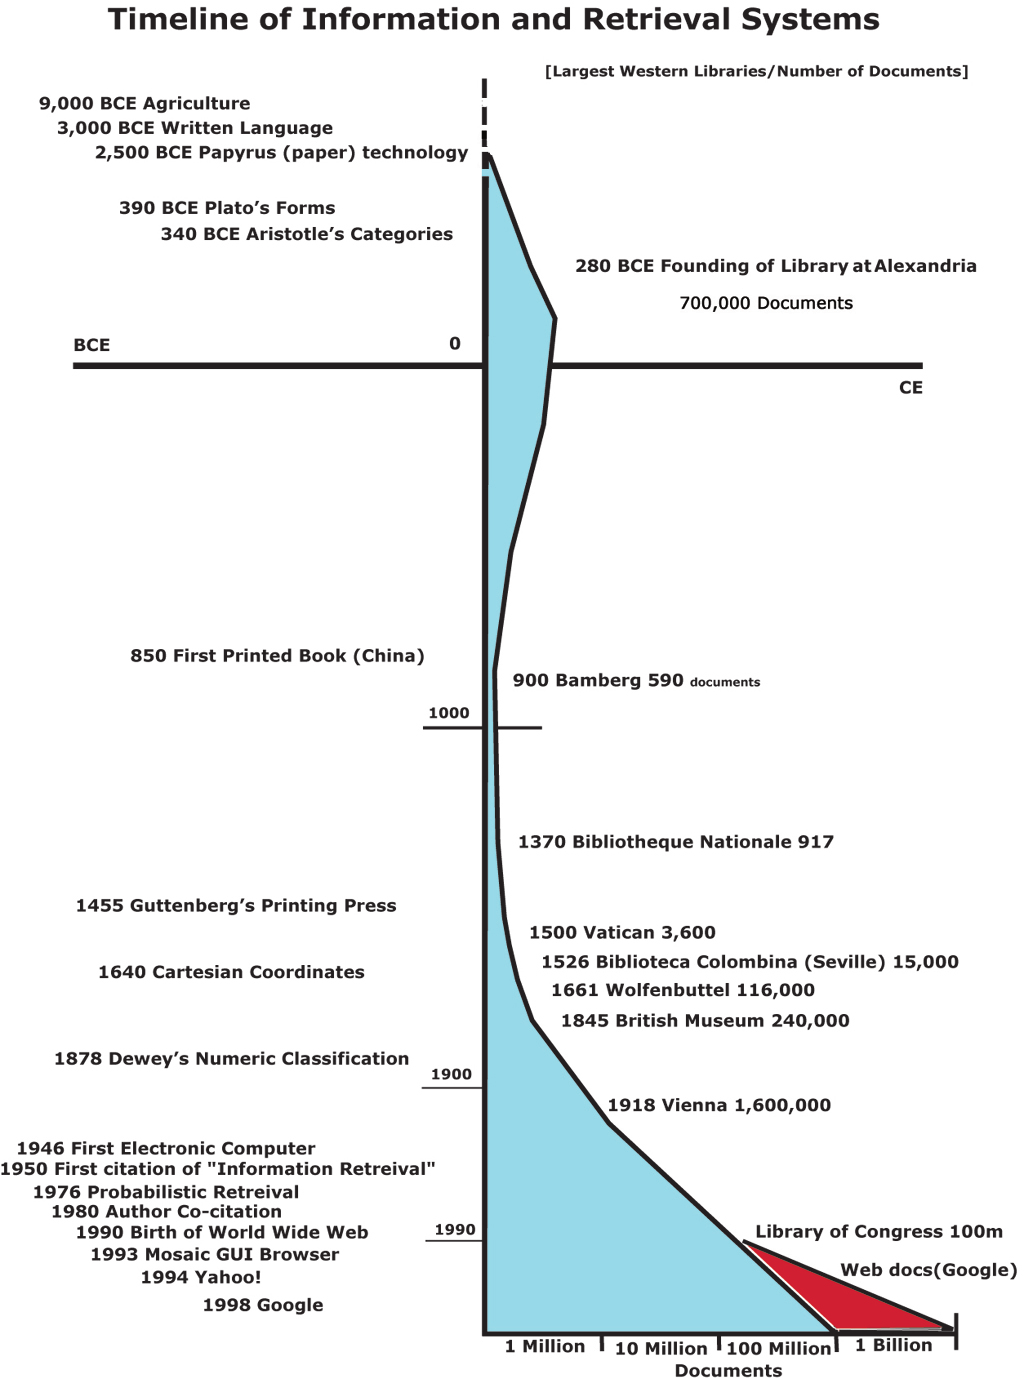
\includegraphics[width=15cm, angle=0]{Figures/RI/ir-history.png}}
    \end{center}
    \caption{Historique de la recherche d'information \citep{ir-course}}\label{fig:ir-history}
\end{figure}

\begin{figure}[htbp]
    \begin{center}
        \fbox{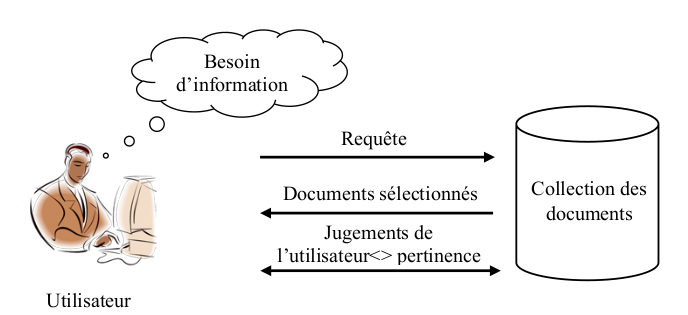
\includegraphics[width=15cm, angle=0]{Figures/RI/processus-ri-simple.png}}
    \end{center}
    \caption{Processus de base de la RI \citep{amelioration-ri-approche-semantique}}\label{fig:processus-ri}
\end{figure}

\section{Information}
\subsection{C'est quoi une information~?}
Une information est issu lorsqu'on donne un sens a un données. Un donnée est donc un unité élémentaire d'information, un octets constitué de bits c'est à dire des 0 et des 1. Un donnée est une représentation a laquelle une signification peur être rattaché, peut être quantitative ou qualitative et n'a pas de sens elle-même.

Une information est donc une collection des données pour donner une forme a une message que ce soit imagée, écrite ou orale pour réduire l’incertitude et transmettre quelque chose qui déclenche une action \citep*{thesaurus-ir-web, construction-memoire-organisationnel-benayache}.

\citeauthor{j-velo:sys-user} \citep{j-velo:sys-user} définit une information comme un fait, une réalité, qui augmente la connaissance des individus. Elle est constitué de \textit{données} et de \textit{sens} qui est attribué par un individu. Le sens dépend de l'individu qui reçoit la données.

\subsection{Pourquoi rechercher de l'information~?}
Lorsqu'un utilisateur a un besoin informationnel (Besoin d'information) la RI est nécessaire pour satisfaire ce besoin. D'où l'initiation de sa Recherche d'information. C'est le besoin d'information de l'utilisateur qui déclenche alors le processus de RI qu'on va voir dans la Section~\ref{sec:besoin-information}.

Le défi de la recherche d'informations est de satisfaire le mieux la demande de l'utilisateur en retournant un ensemble des documents correspondant a ses demandes parmi un grand volume de documents \citep{amelioration-ri-approche-semantique}.

\section{Document}
\subsection{C'est quoi un document~?}
\citeauthor{thesaurus-ir-web} propose quelques définitions d'un document, on va citer deux parmi ceux qui sont cité \citep{thesaurus-ir-web}.

\begin{definition}
    Un document est généralement l'expression d'une pensée humaine.
\end{definition}

\begin{definition}
    Un document représente toute base de connaissance fixé matériellement, susceptible d'être utilisé pour la consultation, l'étude ou la preuve (imprimé, manuscrit, représentation graphique, \dots).
\end{definition}

\begin{definition}
    On appelle document toute unité qui peut constituer une réponse à une requête d'utilisateur. Un document peut être un texte, un morceau de texte, une page Web (HTML), une image, une bande vidéo, sons, etc \citep{salton1989automatique}.
\end{definition}

Un document composé de cinq éléments \citep{thesaurus-ir-web}:
\begin{itemize}
    \item \textbf{Support d'enregistrement}: papier, disque magnétique, CD/DVD-ROM, etc. C'est un support où le document est stocké.
    \item \textbf{Forme d'enregistrement}: papier, codage ASCII, codage vidéos, etc. C'est la forme de document sur le support.
    \item \textbf{Support de restitution}: papier, écran d'ordinateur, haut-parleurs, etc.
    \item \textbf{Forme physique de restitution}: encre sur papier, signal audio ou vidéos, etc.
    \item \textbf{Forme sémantique de restitution}: représentation qui respecte une certaine structure ou forme selon laquelle elle soit intelligible par le l'utilisateur. Écriture, sons, images, animés, etc.
\end{itemize}

Par la suite de ce document, nous traitons principalement des documents textuelles numérique, non structurés.

\subsection{Classification des documents}
\subsubsection{Type de classification des documents}
Pour pouvoir récupérer les documents qui sont similaires, ainsi que pour faciliter le filtre des résultats par l'utilisateur, il est important de classifier les documents.

La classification des documents permet donc de grouper ensemble les documents similaire dans un classe. Cette opération se fait sur la collection des documents ou corpus. Il y a deux types de classification \citep*{modern-ir} tel que la classification \textit{local} et la classification \textit{global}:
\begin{itemize}
    \item \textbf{Classification global}: les documents sont groupés selon leur occurrences dans la collection.
    \item \textbf{Classification local}: les groupement des documents est affecté par le contexte défini par la requête et les documents local sélectionné. La classification varie selon la requête de l'utilisateur.
\end{itemize}

\subsubsection{Algorithmes de classification global}
Diverses algorithmes permettent de classifier les documents textuels, dont certains sont basé sur l'algorithme du \emph{Machine Learning (ML)} et de l'\emph{Intelligence Artificiel (IA)}. Citons quelques algorithmes présenté dans des revue scientifique des classifications des documents textuels \citep*{classification-text-documents,classification-text-documents-ml}.

Pour l'approche du machine learning, il y a des algorithmes qui se base sur l'\emph{apprentissage supervisé}, l'\emph{apprentissage non supervisé} et l'\emph{apprentissage par renforcement}.

\begin{itemize}
    \item \textbf{K-Plus Proche Voisin ou K-Nearest Neighboor (KPP ou KNN)}: Est un approche non paramétrique, utilisé pour classifier des textes. L'approche définit \textit{K} classe pour classifier. Pour décider si $d_{i}$ appartient a la classe $C_{k}$, la similarité ou la dissimilarité pour tous les documents $d_{j}$ dans le donnés d’entraînement est déterminé.
    \item \textbf{Arbre de décision}: La décision est basé sur certains conditions, et utilise un arbre. Les règles de classification sont représentés a travers la chemin du racine au feuille. L'algorithme d'arbre de décision le plus connu est \textit{ID3} et ses successeurs tel que \textit{C4.5} et \textit{C5}. Cette approche a des avantages comme, simple a expliquer et a comprendre par des personnes non connaisseur du domaine, simple a mettre en place ainsi utile dans les analyses prédictives.
    \item \textbf{Naive Bayes Classifier}: Est un algorithme de machine learning, et généralement utilisé pour classifier les documents WEB, qui est un approche probabiliste. Permet de catégoriser des documents, des news, etc. Cette algorithme est efficace, et qui nécessite moins de données d’entraînement, ainsi le résultat est efficace.
    \item \textbf{Support Vector Machine}: Est une approche supervisé du Machine Learning. Le SVM Classifie les données dans différentes classe par la recherche du ligne qui sépare les données d'entrainement en classes, on l'appelle ligne d'hyperplan. Il y a deux catégories tel que le \textit{SVM} linéaire et le \textit{SVM} non linéaire. Cette approche est performant pour classifier les données d’entraînement ainsi corrige bien la classification pour les futures données.
    \item \textbf{D'autres algorithmes}: Il y a d'autres algorithmes pour classifier les documents, mais qui seront pas couvert dans ce travail.
\end{itemize}

\section{Besoin d'information}\label{sec:besoin-information}
\begin{definition}
    C'est la besoin d'information qui déclenche la recherche d'information de l'utilisateur. C'est une sensation qui porterait un individu a s'engager dans une activité de recherche d'information \citep{thesaurus-ir-web}.
\end{definition}

\begin{definition}
    C'est une abstraction mentale dont l'utilisateur a besoin pour répondre a une question ou demande particulière et qui est exprimé en langage naturel \citep{amelioration-ri-approche-semantique} (Reformulation nécessaire).
\end{definition}

C'est cette besoin d'information que l'utilisateur doit traduire pour obtenir une requête afin qu'un SRI puisse satisfaire ce besoin, on dit souvent des mots clés de recherche \citep{modern-ir}.

La besoin d'information se catégorisent en trois types \citep{paradis:tel-00005009} tel que:
\begin{itemize}
    \item[•] \textbf{Besoin vérificatif}: l'utilisateur recherche une donnée particulière, et sait comment y accéder pour vérifier le texte avec des données qu'il possède déjà. En d'autre terme, l'utilisateur possède déjà les données ou la partie mais il a besoin de vérification. Le besoin ne change pas au cours de sa recherche, on dit que c'est \textit{stable}.
    \item[•] \textbf{Besoin thématique connu}: l'utilisateur cherche a éclaircir, revoir ou trouver des nouvelles informations concernant un sujet ou domaine connu. La besoin peut changer (\textit{stable}) ou non (\textit{variable}) au cours de sa recherche ainsi qu'il peut se raffiner. Le besoin peut s'exprimer de façon incomplète.
    \item[•] \textbf{Besoin thématique inconnu}: l'utilisateur cherche des nouveaux concepts ou relations hors des domaines ou sujet connus. La besoin est variable et toujours exprimé de façon incomplète.
\end{itemize}

Pour mieux élaborer ce processus, on va analyser dans la Section~\ref{sec:processus-ri} la processus général de la recherche d'information, la processus en U.

\section{Tâche de recherche de l'utilisateur}
Une tâche de recherche c'est qu'un utilisateur doit faire pour satisfaire un besoin d'information \citep*{boubee-tricot-2010,ri-sur-le-web}.
Les tâches se catégorisent suivant deux types, une tâche \emph{fermé} et une tâche \emph{ouverte}. Une tâche fermé est une tâche dont l'utilisateur cherche une réponse exacte sur une requête donnée, tandis qu'une tâche ouverte est une tâche dont l'utilisateur cherche une réponse acceptable. Après certains études cités dans \citep{ri-sur-le-web} et d'autres chercheurs, que la tâche ouverte utilise d'avantage la navigation, tandis que la tâche fermé privilégie les moteurs de recherche.

\citeauthor{ir-on-web} \citep{ir-on-web} cite deux stratégies de recherche en utilisant des requêtes:
\begin{itemize}
    \item[•] \textbf{Bottom-up ou mixtes:} la recherche commence par une sphère étroite (précise) puis l’élargir de plus en plus. L'utilisateur fait une recherche de plus précise a une recherche plus générale.
    \item[•] \textbf{Top-down:} la recherche commence par une sphère large (générale) puis le rétrécir de plus en plus. L'utilisateur fait une recherche de plus générale a une recherche de plus en plus précise.
\end{itemize}

Selon \citeauthor{ri-sur-le-web} \citep{ri-sur-le-web}, il y a trois type de tâches tel qu'une \textit{tâche factuelle} qui est une tâche généralement fermé, une \textit{tâche interprétative} qui est une tâche généralement ouverte et une \textit{tâche d'exploitation} qui est une tâche complètement ouverte.

\subsection{Tâche factuelle}
Une tâche factuelle est catégorisé dans la tâche fermé, on peut le considérer comme une tâche fermé. Dans une tâche factuelle, les utilisateurs formulent de requêtes dans un SRI ou moteur de recherche, et lisent les résumés de chaque document dans la page de résultat. Ils veulent trouver une réponse sur la page de résultat et privilégie le résumé qui contient les mots clés, et en cliquant juste pour confirmation. Dans cette tâche les experts utilise plutôt la stratégie \emph{bottom-up} tandis que les novices utilisent la stratégie \emph{top-down}.

\subsection{Tâche interprétative}
Une tâche factuelle est catégorisé dans la tâche ouverte, on peut le considérer comme une tâche ouverte. Les utilisateurs commencent par le parcours des informations générales, puis affiner leurs recherche pour leurs besoins spécifiques. Ils privilégié la lecture de contenu des pages et la navigation, souvent une navigation interne a des pages web (via des liens internes) ou externes.

\subsection{Tâche d'exploitation}
Une tâche d'exploitation est une tâche complètement ouverte. Les utilisateurs se concentrent plus sur la page de résultat pour trouver une résultat qui semble correspondre au besoin, puis cliquent et naviguent dans la page pour explorer. Ils veulent trouver de l'information basé sur les contenues de la page. Dans cette tâche, les experts utilisent la stratégie \emph{top-down} tandis que les novices utilisent la stratégie \emph{bottom-up}.

\section{Modèle de recherche de l'utilisateur}
En général il y a deux approche de recherche d'information, dont l'approche classique qui est le \emph{Ad-hoc} et et l'approche moderne qui est le \emph{Filtering} (Filtre en français) \citep{modern-ir}.

\subsection{Ad-hoc: approche classique}
L'approche classique est l'approche la plus utilisée, d'où c'est une approche conventionnel de la Recherche de l'Information. Dans une approche classique, les documents sont resté relativement statique (les documents sont préparés a l'avance). Puis arrivé ensuite la requête des utilisateurs pour trouver une réponses dans ces documents. En d'autre terme, les documents restent statique jusqu’à ce que la requête de l'utilisateur arrive.

\subsection{Filtering: approche moderne}
L'approche moderne consiste a mettre en place un profile complexe de l'utilisateur pour savoir quel documents ou informations pourra lui interrelié. Dans cette approche, les requêtes (préférences, type d'informations qui lui intéressent, \dots) de l'utilisateur restent statique jusqu’à ce qu'un nouveau document arrive dans le système, et que ce système décide si c'est pertinent par rapport au profil de l'utilisateur. Cette approche est souvent utilisé pour les news, marketing, \dots

\section{Facteur d'influence de la recherche d'information}
La recherche d'information de l'utilisateur est influencé par plusieurs facteurs, tel que l'expérience, facteur socio-culturel, et d'autres facteurs.
On peut citer d'après l'analyse de ces facteurs fait par \citeauthor{ri-sur-le-web} \citep{ri-sur-le-web} les facteurs ci-dessous:
\begin{itemize}
    \item \textbf{Expérience de l'utilisateur}: l'expertise du domaine implique la qualité de choix des mots clés a utiliser, la stratégie de recherche; l'expertise du système implique la connaissance de fonctionnement d'un SRI et la stratégie de la RI;l'expertise de la RI implique la capacité d'utiliser un SRI spécifique.
    \item \textbf{Tâche de recherche}: influencé par le type de tâche de l'utilisateur, qu'il recherche de réponse exacte (\textit{tâche fermé}) ou recherche de réponse acceptable (\textit{tâche ouverte}).
    \item \textbf{Facteur socio-culturel}: la contexte sociale et la culture est indissociable de la recherche d'information; le genre influence aussi la recherche, la stratégie de recherche utilisé par les femmes est différente de celle de l'homme, et la chance de réussite est différente; l'âge aussi a son influence, les jeunes et les personnes âgés ont différente façon de faire une recherche. Par exemple, les jeunes on tendance a consulter moins de pages et formuler des requête plus souvent que les âgées.
    \item \textbf{Connaissance de fonctionnement de SRI}: parfois les connaissances sont fausse par rapport aux capacités des moteurs de recherche. L'utilisateur estime qu'il sait utiliser un SRI alors qu'il n'exploite véritablement les capacités du SRI\@.
    \item \textbf{D'autres facteurs}: d'autres facteurs sont aussi détaillés dans la section 2.2.5, comme la limite de temps, caractéristiques individuelles. Un tableau de synthèse de ces facteurs est présenté dans la section 2.3.
\end{itemize}

Pour plus de détails sur ces facteurs d'influences, voir \citetitle[section 2.2]{ri-sur-le-web}

\section{Processus de recherche d'information}\label{sec:processus-ri}
Le modèle de processus le plus utilisé est le modèle en U. C'est un modèle qui traite les documents et la requête séparément et faire une appariement après.

\subsection{Processus en U}
La processus en U se déroule en général quatre étapes \citep{modern-ir} avec deux type de traitement, d'un coté la traitement des documents et de l'autre coté la traitement de la requête. L'\emph{indexation des documents}: créer la base documentaires dans la base de données; \emph{traitement et opérations sur la requête}: traiter la requête de l'utilisateur, retirer les mots vides; l'\emph{appariement de la requête et les documents}: pour savoir quelles documents répond mieux a la requête de l'utilisateur; Et enfin la \emph{reformulation de la requête de l'utilisateur}: pour améliorer les résultats obtenues. La Figure~\ref{fig:processus-u} illustre le processus de la recherche d'information en U.

\begin{figure}[htbp]
    \begin{center}
        \fbox{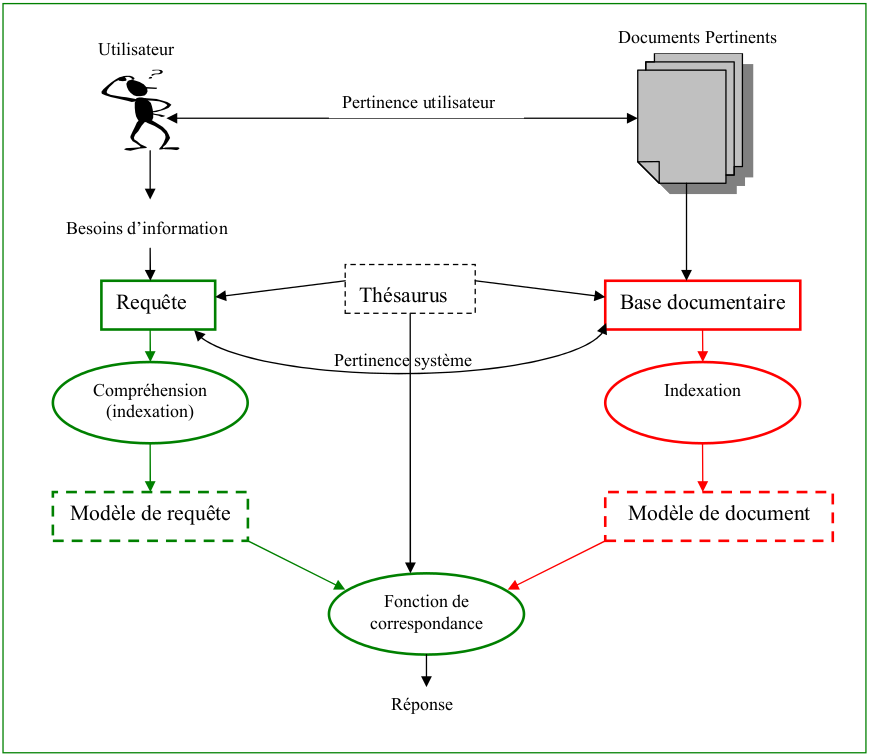
\includegraphics[width=15cm, angle=0]{Figures/RI/Processus-U.png}}
    \end{center}
    \caption{Processus en U de la RI \citep{thesaurus-ir-web}}\label{fig:processus-u}
\end{figure}

Pour la suite, on va expliquer en détails chaque partie de ce processus pour mieux élaborer l'étape de la recherche d'information.

\subsection{Première étape: Besoin d'information}
Comme définit dans la Section~\ref{sec:besoin-information}, pour qu'une recherche d'information eu lieu, il faudra une besoin d'information. A ce stade la base documentaire est déjà mis en place et est déjà prête pour l'utilisation. L'utilisateur doit ensuite transformer son besoin en requête et obtenir des mots clés. Le système applique un traitement de texte (Traitement de Langage Naturel) sur la requête pour obtenir une requête finale qui sera utilisé pour l'appariement. La requête pourra contenir un ou plusieurs mots clés \citep{modern-ir}.

\begin{definition}[Requête ou Query]
    La requête est une interface entre l'utilisateur et le programme, formulé sous-forme des mots-clés par l'utilisateur, décrits en langage naturel \citep{amelioration-ri-approche-semantique}.
\end{definition}

\begin{definition}[Requête ou Query]
    On appelle requête, l'expression du besoin d'information d'un utilisateur. Elle est en général exprimé sous fore des mots clés \citep{salton1989automatique}.
\end{definition}

\subsection{Indexation des documents}
Pour travailler efficacement avec les documents et pour pouvoir rechercher des informations dedans, il faut représenter les documents sous formes des mots clés que contient le document, sous l'approche d'\emph{indexation} \citep{ir-on-web}.

\begin{definition}
    L'indexation est l'action de représenter les contenu des documents sous forme d'index.
\end{definition}

\begin{definition}
    On appelle indexation ou processus d'indexation, le processus qui permet de construire les index a partir de l'analyse du documents tel que la vérification qu'un mot n'est pas dans un anti-dictionnaire (mots vides ou stop words), et la lemmatisation ou racinisation pour trouver la racine des mots. Cette approche est formalisé en utilisant un langage d'indexation. \citep{paradis:tel-00005009}.
\end{definition}

\subsubsection{C'est quoi un index~?}\label{sec:index}
Un index est un mot ou groupe des mots sélectionné soit manuellement par un expert (personne expert du domaine en question), soit automatiquement par un ordinateur (programme informatique) pour représenter un document. Les termes d'indexation sont tous les index qui représentent un document. Un index est en général un nom ou groupe des noms.

Selon Salton, qui traite généralement les index comme représentant du document, Un index est une représentation synthétique de l'information relative a un document, qui met en évidence sa sémantique en vue d'une requête. Selon d'autres auteurs, se sont des mots clés \citep{paradis:tel-00005009}.

\subsubsection{Approche d'indexation}
Comme on a évoqué dans la Section~\ref{sec:index} et cité dans \citep{ir-on-web} ainsi que dans \citep{amelioration-ri-approche-semantique}, il y a en général quatre approche d'indexation tel que l'\textit{indexation manuel}, l'\textit{indexation intelligent}, l’\textit{indexation automatique}, et l'\textit{indexation basé sur les métadonnées}. Il y a une approche \textit{semi-automatique} qui est l'hybridation de l'indexation manuelle et l'indexation automatique, cette approche consiste a créer les index automatiquement puis ces index sont validés par un expert \citep{paradis:tel-00005009}.

\begin{itemize}
    \item[•] \textbf{Indexation manuelle (Human Indexing):} c'est un expert humain qui fait l'indexation. Cette approche a une avantage d'être plus précise en sélection des termes d'indexation. Tandis qu'avec la croissance de volume d'informations, cette approche est de plus en plus obsolète, ainsi il se peut qu'il y a une incohérence entre les experts en sélectionnant les termes d'indexation. De plus cette approche est coûteux \citep{evaluation-of-ir-system}.
    \item[•] \textbf{Indexation automatique (Automatic Indexing):} c'est un programme informatique qui fait l'indexation. Cette approche a une avantage d'être moins coûteux que l'indexation manuel, et résout l'incohérence entre les termes d'indexation sélectionné. Mais peut être moins efficace en sélectionnant les index, les index peuvent être moins précise. Cette approche utilise généralement la Traitement de Langage Naturel (NLP) et de la Statistique (segmentation, suppression des mots vides, etc.).
    \item[•] \textbf{Indexation intelligent (Intelligent Indexing / Agent-Based Indexing):} utilisation des robots (Spiders / Crawlers) pour l'indexation du \emph{WEB}. Un \emph{robot} ou \emph{spiders} est un programme informatique qui parcours les liens sur le web et index les documents trouvées. Cette approche a trois problèmes en général (Robot Standard Exclusion) tel que, les robots peuvent causer des \emph{surcharge au niveau des serveurs}, ils sont \emph{invasives}, et la \emph{mise a jour fréquent des sites web}.
    \item[•] \textbf{Indexation basé sur les métadonnées:} utilisation et interprétation des métadonnées, souvent utilisé dans la recherche d'information sur le web (HTML).
\end{itemize}

Dans le cadre de ce mémoire, on focalisera sur l'indexation automatique des documents textuelle par un programme informatique.

\subsection{Analyse lexical ou Segmentation}
L'analyse lexical des textes permet de faire une analyse de la lexique. Cette analyse peut varier suivant la langue utilisée. On analyse généralement les ponctuations, les espaces entre les mots et la casse des lettres. On considère que la séparation des mots est le caractère espace. L'analyse lexical est alors l'action de convertir les textes du document en groupe des mots (stream of words) qui peuvent être sélectionné comme termes d'indexation. Les nombres sont souvent une mauvaise index sauf s'il est mixé avec un mot. Les expressions régulières sont souvent utiles pour extraire des nombres comme le numéro de carte de crédit, \dots \citep*{modern-ir, approche-semantique}.

\subsubsection*{Ponctuation}
Les ponctuations sont normalement supprimés dans le cas d'analyse lexicales. Sauf dans le cas pour distinguer 'x.id' et 'xid.', la ponctuation ne doit pas être supprimé. \citep{modern-ir}

\subsubsection*{Casse des lettres}
Il faut convertir tous les mots en majuscules ou en minuscules. Mais en particulier, les langages de commande (ligne de commande) de Linux, car l'utilisateur ne veut pas convertir la casse des lettres \citep{modern-ir}. Ça peut perdre aussi l'aspect sémantique après la conversation.

\subsection{Élimination des mots vides (Stop words)}
On appelle un mot vide, un mot qui est plus souvent utilisé dans un document ou dans les termes de recherche d'un utilisateur comme les prépositions, les articles, les conjonctions. Certains verbes, adverbes, et adjectifs pouvant être traité comme mots vides. Éliminer ces mots est important car un mot qui apparaît 80\% dans le corpus n'est pas utile pour la recherche d'information. C'est l'action de supprimer les mots insignifiants (pronoms personnels, préposition, \dots) \citep*{modern-ir, approche-semantique, sarch-engine-vsm}.

Voici une liste non exhaustive des mots vides en français selon \citep{stopwords_french}: le, de, du, mais, donc, car, ceci, cela, qui. A noter que pour un SRI Full-text qui prend tous les mots comme des termes d'indexations, il n'y a pas de suppression des mots vides \citep{modern-ir}.

\subsection{Lemmatisation et Stemming}
La lemmatisation ou racinisation de mot est une partie de le traitement de langage naturel (TLN) qui extrait la racine d'un mot pour regrouper les variants (biologiste, biologique $\rightarrow$  biologie; suis, est $\rightarrow$ être). Cette approche réduit la taille des termes d'indexation \citep*{approche-semantique, sarch-engine-vsm}.

Le Stemming regroupe aussi les variants d'un mot pour obtenir ce qu'on appelle un stem. Un stem est un portion d'un mot restant après la suppression de ses affixes (suffixes, préfixes), la suppression de pluriel, forme gérondif. Cette approche réduit aussi la taille des termes d'indexation. Le stemming ne permet pas de satisfaire la racinisation d'un mot (peut mal déterminer la racine), que certaine moteurs de recherche n'adopte pas le stemming \citep*{modern-ir, vsm}.

Le stemming possède plusieurs techniques, mais on va citer les techniques principaux comme:

\begin{itemize}
    \item[•] \textbf{Table lookup}: regarder le stem dans un table, mais qui est moins pratique en terme de stockage et accessibilité.
    \item[•] \textbf{Porter algorithme}: est une technique simple, intuitive, peut être implémenté efficacement. Cette approche utilise la suppression des affixes.
    \item[•] \textbf{Successeur}: est un approche plus complexe que la suppression des affixes.Se base utilisation des connaissances linguistiques structurés pour identifier les morphes.
    \item[•] \textbf{N-Grams}: est une approche orienté plus vers la classification que stemming. Cette approche se base sur l'identification des diagrammes et trigrammes.
\end{itemize}

D'autres méthodes sont disponibles actuellement comme celle qui se base sur les expressions régulières, \dots

\subsection{Normalisation}
La normalisation permet de classer les termes comme équivalent. Par exemple, le mot U.S.A doit être traité de la même façon que USA.Cette approche de normalisation peut amener a des problèmes \citep{sarch-engine-vsm}.

\subsection{Sélection et pondération des termes}
Comme on dit précédemment, pas tous les mots dans le documents sont significatifs. Sauf pour un moteur de recherche \emph{full-text} qui index tous les termes. Et aussi pas tous les mots on une même degré ou poids d'importance dans un document. D'où la pondération des termes. Pour déterminer le poids d'un terme dans un collection des documents, on utilise en général deux approche: \textit{Term Frequency (TF)} et \textit{Inverse Document Frequency (IDF)}.

\textit{Le TF (Term Frequency)} du terme $t$ dans un document $d$ est le nombre de fois où le terme $t$ apparaît dans le document $d$. C'est la fréquence du ter $t$ dans le document $d$. Plus ce fréquence est important, plus le terme est important pour représenter le document. Cette mesure sera normalisé afin d'éviter d'avoir un poids trop significatifs pour les documents avec beaucoup de contenu, on l'appelle \textit{Normalized Term Frequency}.

\textit{L'IDF (Inverse Document Frequency)} du terme $t$ dans la collection des documents $D$ est le nombre de document dans la collection contenant le terme $t$. C'est le nombre de document où le terme $t$ apparaît dans la collection des documents $D$. Cette approche permet de déterminer l'unicité d'un terme au sein de la collection des documents. Un terme est important si moins de documents la contiennent; un terme qui apparaît dans presque tous les documents n'est pas significatif, et peut être traité comme un mot vide.

La troisième approche qui est la combinaison des deux est la \textit{TF-IDF}. La TF-IDF est la multiplication des deux valeurs obtenues précédemment ($TF*IDF$) pour obtenir le poids final du terme. Le terme est important s'il apparaît dans peu de documents (IDF) mais qu'il apparaît plusieurs fois dans le document qui le contient (TF).

Une fois ces termes sélectionné avec les poids correspondant, on crée un index inversé ou fichier inversé pour stocker ces termes. Cet index inversé va faire correspondre le document identifié par un ID avec les termes qui le compose avec le poids correspondant \citep*{vsm, vsm-for-arabic-language, sarch-engine-vsm, modern-ir}. Tous ces notions va être détaillé un peu plus bas dans le document lorsqu'on abordera le modèle utilisé dans le cadre de ce mémoire.

\subsection{Étape d’appariement}\label{sec:etape-appariement}
Pour pouvoir satisfaire le besoin de l'utilisateur, il faut apparier la requête de l'utilisateur et les documents (fichier inversé) en utilisant un algorithme d'appariement. Ces algorithmes permet de calculer la similarité entre un document et une requête et savoir 
quels sont les documents qui correspondent le mieux avec la requête avec un degré de similarité. Mathématiquement, c'est calculer la distance euclidien entre la requête et le document.

On calcule ces mesures pour déterminer la pertinence entre la requête de l'utilisateur et les documents dans le corpus, on l'appelle \textit{pertinence système}. Il y a aussi le jugement qui provient de l'utilisateur en vue des résultats qu'il obtient par rapport a sa demande, on l'appelle \textit{pertinence utilisateur} \citep{vsm-images}.

La notion de pertinence est très complexe. En général un document est pertinent si l'utilisateur trouve les informations qui satisfait ses besoins dans le document. C'est sur ce notion de pertinence que le SRI doit juger la pertinence. \citep{salton1989automatique}

Les documents trouvés sont retournés a l’utilisateur généralement suivant un degré de pertinence décroissante par rapport a la requête. Certains modèle ne possède pas ce classement des résultats comme le modèle Booléen qu'on va voir dans la section précédente, ainsi que décortiquer ces mesures de similarité.

\subsection{Reformulation de la requête}
La requête de l'utilisateur est parfois courte ou incomplète, alors il faut reformuler la requête par l'ajoute, modification ou suppression des mots clés dans la requête. Il est aussi possible de modifier le poids des termes dans la requête. Parmi les différentes approches proposé, \citeauthor{amelioration-ri-approche-semantique} \citep{amelioration-ri-approche-semantique} note trois approches utilisé dans la reformulation de la requête tel que:

\begin{itemize}
    \item \textbf{Thésaurus}: cette approche utilise une base de connaissance linguistiques pour améliorer la requête de l’utilisateur.
    \item \textbf{Basé sur les co-occurrences}: utilisent le calcul basé sur des co-occurrences des termes.
    \item \textbf{Relevance feed-back}: cette approche se base sur la reformulation de la requête par l'utilisateur par rapport aux pertinences des documents qu'ils reçoivent. En rajoutant, modifiant ou enlevant des termes de recherche ou mots clés.
\end{itemize}

\section{Modèle de RI}
\subsection{Introduction}
Il y a deux raisons pour avoir un modèle dans la recherche d'information. La première, un modèle guide la recherche et donne sens a la discussion académique. La seconde, un modèle est utilisé comme un plan (\emph{blueprint}) pour implémenter un système de recherche d'information \citep{model-ir}.

Un modèle sert a décrire le processus computationnel du RI (comment les documents sont stockés, comment sont stocké les index, etc.), décrire le processus humain (besoin d'information, interaction), ainsi la définition implicite ou explicite de la pertinence \citep{model-ri-cours}.

Pour bien formaliser la recherche d'information, il est nécessaire de définir des modèles a utiliser. L'étape d’appariement dans la Section~\ref{sec:etape-appariement}, nécessite un modèle.

\subsection{Caractéristique formel (DQFR)}
\begin{definition}
    Un modèle de recherche d'information est un quadruplet \emph{DQFR} \citep*{modern-ir, vsm} tel que:
    \begin{itemize}
        \item \textbf{D}: ensemble de représentation (vue logiques) des documents dans la collection.
        \item \textbf{Q}: ensemble de représentation (vue logiques) des besoins de l'utilisateur. On l'appelle requête ou query en anglais.
        \item \textbf{F}: framework pour modéliser les documents, la requête ainsi que leurs relations.
        \item \textbf{R $(q_{i}, d_{j})$}: fonction de classement qui associe un nombre réel avec la requête $q_{i}$ $\in$ \textit{Q} et le document $d_{j}$ $\in$ \textit{D}. Cette classement permet d'ordonner les résultats selon leur pertinence.
    \end{itemize}
\end{definition}

\subsection{Taxonomie de modèle}
Selon \citeauthor{modern-ir} il y a quatre familles principales des modèles de RI qui est illustré dans la Figure~\ref{fig:modele-ri}:

\begin{itemize}
    \item \textbf{Les modèles basé sur les textes du document}: les modèles de RI classique (\textit{Théorie des ensembles, Algébrique, Probabiliste}), et les modèles basé sur le texte semi-structuré (\textit{Texte semi-structuré})
    \item \textbf{Les modèles basé sur le liens entre documents}: les modèles orienté web (\textit{PageRank, Hubs et autorités})
    \item \textbf{Les modèles basé sur les documents multimédia}: les modèles de recherche d'images, vidéos, musiques, etc.
\end{itemize}

\begin{figure}[htbp]
    \begin{center}
        \fbox{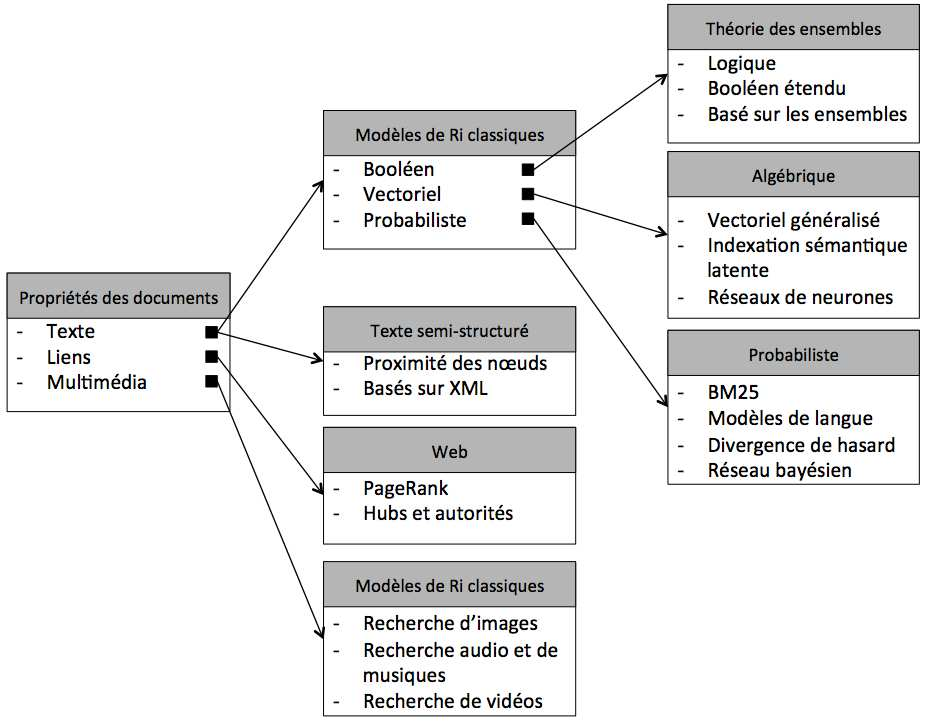
\includegraphics[width=15cm, angle=0]{Figures/RI/modele-ri.png}}
    \end{center}
    \caption{Taxonomie de modèle de RI \citep{soulier2014:def-evaluation-modele}}\label{fig:modele-ri}
\end{figure}

Dans le cadre de ce mémoire, on va analyser la famille des modèles classiques basé sur les textes du document.

\subsection{Catégorie de modèle}
Dans cette famille \citep*{modern-ir, approche-semantique, soulier2014:def-evaluation-modele}, il y a trois grandes catégories des modèles: le modèle \emph{théorique ou ensembliste} (theoretic), le modèle \emph{algébrique} (algrebraic) et le modèle \emph{probabiliste} (probabilistic).

Dans le modèle ensembliste, on trouve principalement le modèle \emph{Booléen}, le modèle \emph{Booléen étendue}. Dans le modèle algébrique, on trouve principalement le modèle \emph{vectoriel} (Vector Space Model), le modèle de \emph{réseau de neurone} (Neural Network Models), et d'autres modèles. Dans le modèle probabiliste, on trouve principalement le modèle probabiliste (Probabilistic model), le \emph{réseau d'inférence} (Inference Network) et d'autres modèles.

Ces modèles sont des modèles de recherche, mais il y a aussi des modèles pour la navigation (Browsing) \citep{modern-ir}.

\subsection{Modèle ensembliste}
\subsubsection{Modèle Booléen (Boolean Model)}
Un exemple de requête dans le modèle Booléen est illustré sur la Figure~\ref{fig:boolean-model}.

\begin{figure}[htbp]
    \begin{center}
        \fbox{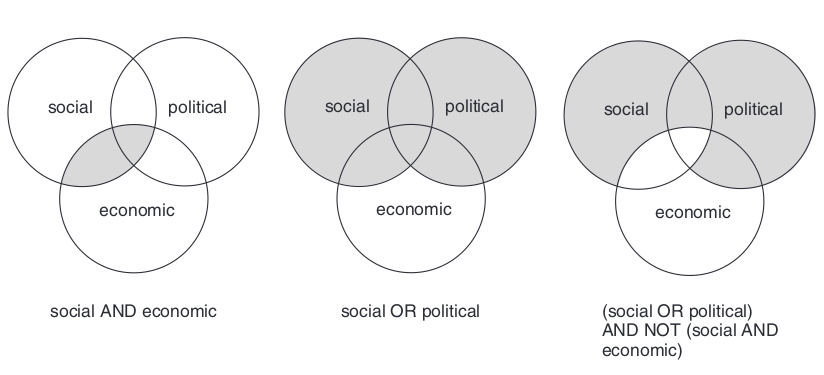
\includegraphics[width=15cm, angle=0]{Figures/RI/boolean-model-example.png}}
    \end{center}
    \caption{Exemple de diagramme de requête \citep{model-ir}}\label{fig:boolean-model}
\end{figure}

C'est un modèle de base, et le premier modèle utilisé dans la recherche d'information. Dans ce modèle, les documents et la requête sont représentés sous forme des mots clés. Ainsi la requête est exprimé en utilisant les opérateurs booléens \emph{ET (AND)}, \emph{OU (OR)} et \emph{NON (NOT)}. La stratégie de recherche est basé sur la décision binaire. Tous les termes d'indexation ont la même poids et qui sont pondérés de façon binaire, soit il existe dans le document soit non. S'il existe dans le document, son poids est 1, sinon 0. La similarité entre $q$ et $d_{j}$ est égal a 1 si le document $d_{j}$ valide l'expression booléen $q$, sinon 0. Un document est donc jugé pertinent par le système s'il valide l'expression booléen de la requête.

Ce modèle a des avantages d'être facile a mettre en place, simple (utilise l'algèbre de Boole) et exacte au niveau des résultats. Ce pour cette exactitude que ce modèle est aussi un modèle exacte (Exact Match Model).

Par contre, ce modèle a des lacunes, il est difficile de transformer le besoin d'information en expressions booléen surtout pour un \emph{utilisateur lambda} (un utilisateur qui ne sait absolument rien de l'expression booléen) donc la requête a tendance un peu simplifié ou même incomplète ce qui affecte la qualité des résultats. Et puisque la décision est binaire, et que le poids soit $1$ soit $0$, il n'y a pas de classement possible pour les documents retournés. L'utilisateur est alors obligé de parcourir les résultats pour juger la pertinence. Puisque le modèle est exacte, le modèle ne permet pas de sélectionner les documents qui peuvent intéressé l'utilisateur et qui peuvent être pertinent par rapport a ses requête, et qu'il est impossible de récupérer une réponses partielles qui valide certains expression de la requête. \citep*{modern-ir, soulier2014:def-evaluation-modele}.

\begin{definition}[Modèle booléen]
    On note $w_{ij} \in \{0, 1\}$ le poids du terme numéro $i$ dans le document numéro $j$ qui est binaire $ \vec{q}_{dnf} $, forme normal de disjonction de la requête $ q $. Considérons $ \vec{q}_{cc} $ composant conjonctive de $ \vec{q}_{dnf} $. La similarité du document $ d_{j} $ par rapport a la requête $ q $ est définie par:

    \[
        Sim(d_{j}, q) = \left\{
        \begin{array}{ll}
            0 & Sinon \\
            1 & \textit{S'il } \exists \vec{q}_{cc} \mid (\vec{q}_{cc} \in \vec{q}_{dnf}) \bigwedge (\forall k_{i}, g(\vec{d_{j}}) = g_{i}(\vec{q}_{cc}))
        \end{array}
        \right.
    \]

    Si $ Sim(d_{j}, q) = 1$, le document $ d_{j} $ est pertinent a la requête $ q $; dans le cas contraire, le document n'est pas pertinent par rapport a la requête.
\end{definition}

\subsubsection{Modèle Booléen Étendu (Extended Boolean Model)}
En vue de ces lacunes, le modèle booléen est amélioré afin de résoudre certains problèmes avec le modèle Booléen. Premièrement, le modèle Booléen étendue a mis en place la possibilité de faire une similarité partiel et la pondération des termes. Il est étendu en ajoutant la fonctionnalité du modèle vectoriel qui est la combinaison de formulation de requête avec les caractéristiques du modèle vectoriel. Ce modèle est introduit par \citeauthor{salton1983étendu} \citep{salton1983étendu} en 1983. Mais ce modèle n'a pas été largement utilisé \citep{modern-ir}.

\subsubsection{D'autres modèles}
Il y a aussi d'autres modèles dans la catégorie ensembliste, tel que le modèle de Fuzzy (Fuzzy Set Model, Region Models), \dots, mais qui ne sont pas détaillé dans le cadre de ce mémoire. Pour plus de détails, voir chapitre 2 \citep{modern-ir} et chapitre 1 \citep{model-ir}.

\subsection{Modèle algébrique}
\subsubsection{Modèle Vectoriel (Vector Space Model)}\label{sec:vsm-model}
Ce modèle a un alternative qui est le \emph{Modèle Vectoriel Généralisé} par \citeauthor{salton1975vector} \citep{salton1975vector}, qui se base sur des vecteurs. Les documents et la requête sont représentés par un vecteur dans un \emph{t-espace vectoriel} (représentation algébrique). Ce modèle accorde une appariement partielle, et les termes ne sont pas pondérés de manières binaires. Les pondérations des termes le plus souvent utilisé sont la \emph{TF}, \emph{IDF}, et la \emph{TF-IDF} \citep*{sarch-engine-vsm}.

Un score de similarité est alors exprimé comme un mesure de proximité entre deux entités correspondant a l'angle qui sépare les deux vecteurs. Ces mesures sont présentés dans la Section~\ref{sec:mesure-similarite}.

\begin{figure}[htbp]
    \begin{center}
        \fbox{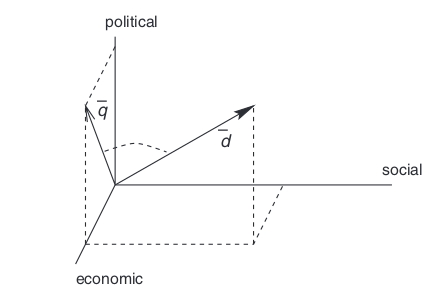
\includegraphics[width=10cm, angle=0]{Figures/RI/vector-model.png}}
    \end{center}
    \caption{Représentation du document et la requête \citep{model-ir}}\label{fig:vector-model}
\end{figure}

Le modèle vectoriel a certains avantages comme la facilité mise en œuvre, la possibilité d'avoir un appariement approximatif avec un degré de pertinence (l'utilisateur reçoit des documents qui pourrait lui intéressé), la possibilité d'organiser les résultats suivant leur pertinence (l'utilisateur passe moins de temps a filtrer les résultats puisqu'ils sont déjà ordonné), ainsi le pouvoir de définir une limité pour la mesure de similarité et de n'afficher que les documents qui sont en dessus de cette limite pour éliminer les résultats le moins pertinent. Ce modèle est populaire, et le plus utilisé par les moteurs de recherche actuel. \citep*{approche-semantique, modern-ir, soulier2014:def-evaluation-modele}

Par contre, l’indépendance des termes d'indexation implique la perte de la notion de sémantique du document. Mais ce problème a été solutionné par la mise place de regroupement des termes qui ont la même sens, on l'appelle \emph{N-grammes}. Ou bien une autre approche est d'utiliser le modèle d’\emph{indexation sémantique} latente (Latent Semantic Index).

\begin{definition}[Modèle Véctoriel]
    On note $w_{ij}$ le poids positif et non binaire, du terme $i$ dans le document $j$ qui est associé avec un pair $(k_{i}, d_{j})$ et $w_{iq}$ le poids du terme $i$ dans la requête $q$. La requête est définie par le vecteur: $ \vec{q} = (w_{1q}, w_{2q}, \dots, w_{tq}) $ où $t$ le nombre total des termes d'indexation dans le système. Un document $d_{j}$ est présenté par le vecteur: $ \vec{d_{j}} = (w_{1j}, w_{2j}, \dots, w_{tj}) $.

    La calcul de similarité entre ces deux vecteurs se traduit par la formule:
    \[
        Sim(\vec{d}, \vec{q}) = \frac{\vec{d_{j}} \cdot \vec{q}}{ |\vec{d_{j}}| \times |\vec{q}| } \\
        = \frac{\sum_{i=1}^{t} w_{i,j} \times w_{i,q}}{\sqrt{\sum_{i=1}^{t} (w_{i,j})^2} \times \sqrt{\sum_{i=1}^{t} (w_{i,q})^2}}
    \]

    Avec $ |\vec{d_{j}}| $ et $ |\vec{q}| $ norme du vecteur document et de la vecteur requête.
\end{definition}

\subsubsection{Autre modèle}
Il y a d'autres modèles dans la catégorie algébrique tel que le modèle d'Indexation Sémantique Latente (Latent Semantic Indexing) et le modèle de réseau de neurones (Neural Network Model).

L'approche d'indexation sémantique latente est introduit en 1988, qui permet de garder la sémantique des documents pour avoir une relation entre les termes d'indexation. Cette approche se base sur l’appariement de contexte au lieu d'index, voir \citetitle[Page 45]{modern-ir} \citep{modern-ir} pour les détails complet.

Le modèle neuronale se base sur des processus d'activation des neurones (spread activation process), cette approche est plus orienté vers l’intelligence artificielle \citep*{modern-ir}.

\subsection{Modèle probabiliste}
Dans le modèle probabiliste, le framework pour modéliser les documents et la représentation de la requête se base sur la théorie des probabilités. Les détails seront présentés dans \citetitle[Section 2]{modern-ir} \citep{modern-ir}.

\subsubsection{Modèle probabiliste}
\begin{figure}[htbp]
    \begin{center}
        \fbox{
\includegraphics[width=15cm, angle=0]{Figures/RI/probabilistic-model.png}}
    \end{center}
    \caption{Diagramme de collection pour le terme \emph{social} \citep{model-ir}}\label{fig:probabilistic-model}
\end{figure}

Le principe du modèle probabiliste est de donner la requête $q$ de l'utilisateur et un document $d_{j}$ dans la collection. Puis le modèle estime la probabilité que l'utilisateur trouve le document $d_{j}$ pertinent. Le modèle assume que ce probabilité de pertinence dépend seulement de la requête et la représentation du document. La mesure de similarité utilise la \emph{formule de Bayes} (Bayes's rule). Les détails sont présentés dans \citetitle[Section 2]{model-ir} \citep{model-ir} et \citetitle[Section 1.4]{modern-ir} \citep{modern-ir}.

\begin{definition}[Modèle probabiliste]
    On note $w_{ij} \in \{0, 1\}$ le poids du terme $i$ dans le document $j$, et $w_{iq} \in \{0, 1\}$ le poids du terme $i$ dans la requête $q$.\\
    $R$: Ensemble des documents connu ou initialement estimé d'être pertinent.\\
    $\bar{R}$: Complément de $R$, l'ensemble de documents non pertinent.\\
    $P(R/d_{j})$: Probabilité de pertinence du document $d_{j}$ pour la requête $q$. \\
    $P(\bar{R}/d_{j})$: Probabilité de non pertinence du document $d_{j}$ pour la requête $q$.

    \[
        Sim(d_{j}, q) = \frac{ P(R/\vec{d_{j}}) }{ P(\bar{R}/\vec{d_{j}}) } = \frac{P(\vec{d_{j}}/R) \times P(R)}{P(\vec{d_{j}}/\bar{R}) \times P(\bar{R})}
    \]

    Où:\\
    $ P(d_{j}/R) $: Probabilité de sélection du document $ d_{j} $ au hasard provenant de l'ensemble $ R $ des documents pertinents.\\
    $ P(R) $: Probabilité qu'un document sélectionné au hasard dans la collection entière est pertinent.

    Or, $ P(R) $ et $ P(\bar{R}) $ est la même pour tous les documents, alors la formule de similarité devient:
    
    \[
        Sim(d_{j}, q) \sim \frac{P(\vec{d_{j}}/R)}{P(\vec{d_{j}}/\bar{R})}
    \]

    Avec l'application des poids de terme, la formule de similarité final est donc:
    \[
        Sim(d_{j}, q) \sim \sum_{i = 1}^{t} (w_{iq} \times w_{ij}) \times \left(
            \log{\frac{P(k_{i}/R)}{1 - P(k_{i}/R)}} + \log{\frac{P(k_{i}/\bar{R})}{1 - P(k_{i}/\bar{R})}}
        \right)
    \]

    Tel qu'au départ:\\
    $ P(k_{i}/R) $: $ 0.5 $ \\
    $ P(k_{i}/R) = \frac{n_{i}}{N} $ avec $ n_{i} $ le nombre de documents qui contient le terme $ k_{i} $, et $ N $ le nombre total des documents.
\end{definition}

Ce modèle a un avantage d'avoir le classement des résultats suivant leur probabilité d'être pertinent dans l'ordre décroisant. Par contre, il a quelques lacunes tel que le besoin de savoir initialement la séparation des documents en ensembles pertinent et non pertinent, le modèle ne prend pas en compte le fréquence de terme dans un document ce qui implique que tous les poids des termes sont binaire, ainsi les termes d'indexation sont indépendants \citep{modern-ir}.

\subsubsection{Autres modèles}
Il y a d'autres modèles dans ce catégorie, qui ne sont pas détaillé dans le cadre de ce devoir, comme le \emph{Réseau d'Inférence} (Inference Network), \emph{Réseau Bayésien} (Bayesian Network), le modèle de \emph{Poisson} (The 2-Poisson model) \citep{model-ir}.

\section{Mesure de similarité}\label{sec:mesure-similarite}
Citons quelques méthode de similarité \citep*{vsm-for-arabic-language, sarch-engine-vsm, vsm}:
\begin{itemize}
    \item[•] \textbf{Produit scalaire (Dot Product)}: c'est le produit scalaire entre deux vecteurs. La requête et les documents sont représenté par des vecteurs de même dimension.
    \item[•] \textbf{Similarité cosinus (Cosine Similarity)}: c'est la mesure le plus populaire. Utilise le produit scalaire ainsi que l'angle formé entre les deux vecteurs (document et requête)
    \item[•] \textbf{Coefficient de Jaccard (Jaccard Coefficient)}: mesure statistique de similarité entre des collections (sample set)
    \item[•] \textbf{Coefficient de Dice (Dice Coefficient)}: même que celle de Jaccard, mais double le poids de vecteur
\end{itemize}

Puisque nous nous focaliserons sur le modèle vectoriel dans le cadre de ce mémoire, les quatre principaux mesures de similarité présenté dans la Section~\ref{sec:etape-appariement} sont les mesures utilisés dans le modèle vectoriel. Ces mesures sont utilisé pour déterminer la pertinence système c'est a dire la pertinence des documents par rapport a la requête de l'utilisateur. A bien noter que tous les poids des termes d'indexation sont normalisé avec TF-IDF avant la calcul de ces mesures. Ces mesures sont optionnelles, mais la mesure de similarité le plus populaire est celle de \emph{cosinus} \citep{vsm}.

La pondération des termes se traduit alors comme suit:
\[
    d_{k} = q_{k} = tf(k, d) \cdot \log{\frac{N}{df{(k)}}}
\]

Avec:
Term Frequency (TF):
\[
    TF(k, d) = \frac{\textit{Nombre d'occurences du terme k} \textit{ dans le document d}}{\textit{Nombre total des termes dans le document d}}
\]

Inverse Document Frequency (IDF):
\[
    IDF(t, D) = \log\frac{\textit{Nombre total des documents dans le corpus } N}{\textit{Nombre de documents qui contient le terme } t}
\]

Term Frequency-Inverse Document Frequency (TF-IDF):
\[
    TF-IDF(t, d, D) = \textit{TF}(t, d) \times \textit{IDF}(t, D)
\]

\subsection{Produit scalaire}
Le produit scalaire ou Dot product (Inner Product) en anglais est la mesure de base, qui est utilisé dans d'autres mesure comme celle de cosinus, Jaccard ainsi que Dice. Cette mesure calcul le produit scalaire entre le vecteur document et la vecteur requête. La formule pour calculer ce mesure est ci-dessous:

\[
    Inner Product(\mathbf{A}, \mathbf{B}) = \mathbf{A} \cdot \mathbf{B}
\]

\subsection{Similarité cosinus}
La mesure cosinus ou Cosine Similarity est la mesure la plus populaire. Cette mesure utilise le produit scalaire en introduisant l'angle formé par les deux vecteur (document et requête). La formule pour calculer cette mesure est ci-dessous:

\[
    Sim(\vec{d}, \vec{q}) = \frac{\vec{d} \cdot \vec{q}}{\|\vec{d}\| \cdot \|\vec{q}\|} = \frac{\sum_{k=1}^{n} d_{k} \cdot q_{k}}{\sqrt{\sum_{k=1}^{n} (d_{k})^2} \cdot \sqrt{\sum_{k=1}^{n} (q_{k})^2}}
\]

\subsection{Similarité de Jaccard}
La mesure de Jaccard ou Jaccard's Similarity utilise aussi le produit scalaire, c'est une mesure basé sur la statistique. La formule pour calculer cette mesure est ci-dessous:

\[
    \textit{Jaccard Similarity}(A, B) = \frac{|A \cap B|}{|A \cup B|}
\]

\subsection{Similarité de Dice}
La \emph{mesure de Dice} ou \emph{Dice's Similarity} est la mesure utilise le produit scalaire. La formule pour calculer cette mesure est ci-dessous:

\[
    \textit{Dice Similarity}(A, B) = \frac{2 |A \cap B|}{|A| + |B|}
\]

\section{Conclusion}
La recherche d'information (RI) est une domaine vaste, intéressant mai aussi a des défis comme pour la partie indexation, etc. Elle est ancienne mais a connu beaucoup d'évolution, avec l'explosion de volume d'information disponible sur internet par le biais des réseau sociaux, des blogs, ainsi qu'avec l'arrivée de l'intelligence artificielle ainsi que del la Machine Learning (ML). Elle propose différentes modèles mathématiques qui sont adaptés suivant les types de document (textuelle, image, etc.) pour formaliser la recherche, pour définir la mesure de pertinence entre le document et la requête, qui pourront être améliorer en utilisant les algorithmes de l'intelligence artificielle.

Dans la partie suivante, on va analyser comment ces modèles seront utilisé a travers un Système de Recherche d'information.

\chapter{Système de recherche d'information}
\section{Introduction}
Dans cette section, on va voire d'abord quelques définitions tiré des travaux de quelques chercheurs qui s'y intéressaient dans le domaine de la Recherche d'information et d'un encyclopédie, puis on va analyser ses composant et les types, et enfin on va voir comment analyser la performance d'un moteur de recherche et les mesures de performance souvent utilisé.

\begin{definition}
    Selon \citeauthor{salton1989automatique}, un système de recherche d'information (RI) est un système qui permet de retrouver les documents pertinents à une requête d'utilisateur, à partir d'une base de documents volumineuse \citep{salton1989automatique}.
\end{definition}

\begin{definition}
	On appelle Système de Recherche d'Information (SRI) un ensemble des programmes, qui sert a interfacer avec l'utilisateur, de prendre les requêtes et de les interpréter afin de faire une recherche dans l'index, appliquer un modèle d’appariement et retourné les documents jugés pertinents a l'utilisateur \citep{amelioration-ri-approche-semantique}.
\end{definition}

\begin{definition}
	On appelle SRI ou moteur de recherche, un ensemble de programmes informatiques, qui met en œuvre des techniques et moyens pour trouver les documents pertinents afin de satisfaire le besoin d'information de l'utilisateur. En d'autres termes, permet de retrouver des informations grâce a l'utilisation des mots clés et termes de recherche \citep{approche-semantique}.
\end{definition}

\begin{definition}
	Un Système de Recherche d'Information permet de récupérer la requête de l'utilisateur, de l'analyser, puis rechercher dans la base documentaire les documents qui correspondent (pertinent) a la requête et de retourner les résultats a l'utilisateur \citep{vsm}.
\end{definition}

\begin{definition}
	Un moteur de recherche est un outil qui permet de rechercher sur le Web ou sur un ordinateur personnel des ressources, des contenus, des documents etc., à partir de mots clés \citep{jdn-moteur-de-recherche}.
\end{definition}

\begin{definition}
	Un moteur de recherche est un système logiciel qui collecte des informations à partir des ressources documentaires (World Wide Web, \dots) et qui les présente aux utilisateurs qui recherchent des informations spécifiques \citep{mdn-search-engine}.
\end{definition}

\section{Objectif et efficacité}
En général il y a deux catégorie de problème tel que le problème \textit{centré utilisateur} qui est le problème lié a la compréhension et l'analyse de comportement de l'utilisateur; et le problème \textit{centré système} qui est le problème lié a la création d'index efficace, traitements des requêtes avec plus de rapidité et efficacité ainsi que le développement d'un algorithme de classement pour améliorer les résultats \citep{modern-ir}. Mais le problème central d'un SRI se concentre sur le coté système (\textit{centré système}) qui est de savoir comment satisfaire la besoin d'information de l'utilisateur le plus rapide possible et efficace. C'est un problème plus délicat a résoudre puisqu'il y en a plusieurs facteurs relié a ces performances. Mais il y a des recherches qui traite (analyse) les comportement de l'utilisateur ainsi que ses impactes sur la recherche d’information et l'utilisation d'un SRI. Parmi ces différentes études, il y a celle qui est traité par \citeauthor{ri-sur-le-web} \citep{ri-sur-le-web} dans le cadre des lycéens.

L'objectif d'un SRI est donc de localiser et retourner les documents pertinents par rapport a une requête pour répondre et satisfaire le besoin d'information de l'utilisateur. Le SRI relève donc le défi de rechercher des documents pertinents par rapport au requête de l'utilisateur parmi un très grand volume d'informations \citep{amelioration-ri-approche-semantique}.

L'efficacité d'un SRI est jugé par la capacité de comprendre ce que l'utilisateur veut, ce que l'utilisateur demande a partir de la requête. Ainsi sur sa capacité de fournir les documents pertinents et les classer suivant leurs pertinences par rapport a la requête de l'utilisateur \citep{vsm}. Et aussi la rapidité de récupération des informations et l'accessibilité au niveau de l'interface utilisateur \citep{ir-on-web}.

Pour notre cas, on se focalisera plus sur la performance relié au problème centré système que ceux qui est centré utilisateur.

\section{Élément principaux}
Un Système de Recherche d'Information a systématiquement deux éléments principaux, tel que la \textit{base de donnée} et l'\textit{algorithme de classement} \citep{approche-semantique}. Ces deux éléments sont indispensables pour un système d'information.

\subsection{Base de données}
\begin{definition}
	Une base de données est une collection organisée d’informations structurées, généralement stockées
	électroniquement dans un système informatique. Généralement contrôlée par un SGBD (Système de Gestion de Base de Données) \citep{oracle-database}.
\end{definition}

\begin{definition}
	Une base de données ou BDD est une collection d’informations organisées afin d’être facilement consultables, gérables et mises à jour. Les bases de données informatiques sont utilisées dans un grand nombre d’entreprises pour stocker, organiser et analyser les données \citep{lebigdata}.
\end{definition}

\begin{definition}
	Une base de données permet de stocker et de retrouver des données structurées, semi-structurées ou des données brutes ou de l'information, souvent en rapport avec un thème ou une activité \citep{wiki-database}.
\end{definition}

Pour un SRI, cette base de données est structuré par un expert en base de données (Database Manager). Il est responsable de stockage des documents, des index, ainsi que met en place la relation entre les documents et les index (Fichier inversé). Cette base de données stocke alors l'ensemble de documents utilisé par le système afin de répondre aux besoins de l'utilisateur \citep{vsm-for-arabic-language}.

\subsection{Algorithme de classement}
Un algorithme de classement permet de classer les documents suivant l'ordre de pertinence par rapport a la requête de l'utilisateur. Cette algorithme qui se charge de calculer la pertinence entre la requête et les documents dans la base de données. L'algorithme de classement souvent utilisé dans le modèle vectoriel est déjà présenté dans la section \ref{sec:mesure-similarite}.

\section{Catégorie de recherche}
Tout d'abord, il y a quatre catégories de recherche cité par \citeauthor{ir-on-web} \citep{ir-on-web} tel que:
\begin{itemize}
	\item \textbf{Recherche simple}: utilise la requête simple
	\item \textbf{Recherche personnalisée}: utilise la requête personnalisée
	\item \textbf{Recherche de dossier}: recherche dans de dossier
	\item \textbf{Recherche des nouvelles courantes}: utilise la requête des news
	\item \textbf{Contenu web}: suppression des liens mortes
\end{itemize}

\section{Type de moteur de recherche}
Les moteurs de recherche sont catégorisé en deux catégories: moteur de recherche classique qui travaille avec les contenues statique des documents et le moteur de recherche sémantique \citep*{approche-semantique,thesaurus-ir-web}.

Ci-dessous un tableau qui illustre la différence entre un moteur de recherche classique et moderne \citep{ir-on-web} (A analyser si ce tableau est vraiment nécessaire).

\subsection{Classique ou traditionnel}
Un moteur de recherche classique ou traditionnel traite les documents dont le contenu est statique. Le contenu des documents ne change pas au fil du temps. Ce qui veut dire que l'étape d'indexation des documents se fait une fois, il n'y a probablement pas de réindexation des documents. Cette approche est souvent utilisé pour la recherche des livres électronique, etc.

\subsection{Sémantique ou moderne}
Ce moteur de recherche provient du traditionnel. Le contenu des documents traités par ce type de SRI sont dynamiques et peuvent varier au fil du temps. Comme par exemple un site WEB qui met a jour fréquemment ses contenus, modifié ou supprimé. Dans de type de SRI, l'étape d'indexation est de plus en plus complexe, et l'étape de réindexation est nécessaire et souvent periodique pour récupérer les mise a jours des documents. Ce type de moteur de recherche est généralement utilisé pour la recherche sur le WEB.

\section{Modèle adopté par un SRI}
Un Système de Recherche d'Information peut adopter un modèle qui se base sur ces trois modèles qui est le modèle \textit{full-text}, le modèle \textit{keyword-based} et le modèle \textit{hypertext} \citep{modern-ir}.
\begin{itemize}
	\item \textbf{Full-text}: ce modèle utilise tous les termes de documents comme un terme d'indexation. C'est à dire pas de discrimination des mots vides. L'indexation et la tache de recherche sont simple, mais peut apporter des bruits.
	\item \textbf{Keyword-based}: ce modèle utilise les mots clés pour représenter les documents, avec la suppression des mots vides. Les termes d'indexation sont donc des mots clés.
	\item \textbf{Hypertext}: ce modèle se base sur des liens, souvent utilisé sur les documents WEB.
\end{itemize}

\section{Évaluation d'un SRI}
Dans cette section, on va analyser comment bien définir la performance et évaluer un SRI. Il est important d’évaluer un SRI avant d’implémentation pour l'utilisation finale. Cette étape d'évaluation dépend du but finale du SRI. Généralement, il y a quatre trois catégories d'évaluation d'un SRI: \textit{évaluation fonctionnel} qui fait l'analyse des fonctionnalités du système, \textit{évaluation de performance} et l'\textit{évaluation de performance de recherche} \citep{modern-ir}.

Dans ce troisième catégorie, on utilise des mesures mathématique dont les plus courant sont \textit{Précision (Precision)} et \textit{Rappel (Recall)}.

Souvent dans l'étape d'évaluation, l'\textit{évaluation de performance de recherche} est plus difficile et compliqué, qui a un grand défi.

\subsection{Évaluation fonctionnel}
L'évaluation fonctionnel est la première étape d'évaluation d'un SRI. Il met en œuvre l'analyse des deux facteurs suivantes:
\begin{itemize}
	\item \textbf{Analyse de fonctionnalités}: analyser tous les fonctionnalités du système une par une pour voir s'il y a bien des failles ou bug. Cette analyse assurera que l'utilisateur finale du système faire face a des problèmes de fonctionnalités ou bug (analyse de l'interface graphique si c'est conviviale, l'accessibilité, etc.).
	\item \textbf{Analyse d’erreur}: pour l'analyse d'erreur, on cherche a trouver un moyen pour faire échouer le système, trouver par tous les moyens de faire des traitements pour que le système fait un erreur. Cette analyse permet de voir des erreurs qui ne sont pas identifié avant et de pouvoir les corriger après.
\end{itemize}

\subsection{Évaluation de performance}
L'évaluation de performance permet d'identifier la performance et la robustesse d'un SRI. Cette évaluation analyse généralement deux facteurs:
\begin{itemize}
	\item \textbf{Analyse de temps de réponse}: analyser le temps de réponse du système pour répondre a une requête de l'utilisateur. Le but est de minimiser ce temps de réponse pour satisfaire l'utilisateur. Le système doit être rapide en terme de réponse. Avec les machines de plus en plus performants, cet analyse est de moins en moins problématique mais a ne pas ignorer.
	\item \textbf{Analyse de l’espace utilisé}: analyser aussi l'espace disque utiliser par le stockage des index et la collection des documents. Le système doit utiliser le moins d’espace possible, et doit être le plus léger possible.
\end{itemize}

Dans cette évaluation, on analyse aussi la performance d'indexation du SRI, l’interaction avec le Système d'Exploitation, ainsi que le délais dans le canaux de communication.

\subsection{Évaluation de performance de recherche}
L'évaluation de performance de recherche possède un grand défi, est qui est généralement traité par des chercheurs. Le but est de maximiser la précision des résultats de recherche par rapport au requête de l'utilisateur. Pour bien assimiler cette partie, on va voir comment est structuré la collection des documents du point de vue du système, on va illustrer ce qu'on appelle matrice de contingence dans la Figure~\ref{fig:matrice-contingence}.

\begin{figure}[htbp]
	\begin{center}
		\fbox{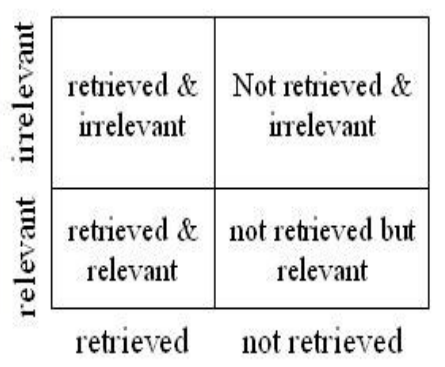
\includegraphics[width=10cm, angle=0]{Figures/matrice-contingence.png}}
	\end{center}
	\caption{Matrice de contingence \citep{vsm-for-arabic-language}}
	\label{fig:matrice-contingence}
\end{figure}

Dans ce matrice, il y a quatre catégories tel que:
\begin{itemize}
	\item \textbf{Récupéré et non pertinents}: se sont des documents non pertinents mais jugés pertinent par le système. On cherche a minimiser le nombre des documents dans cette catégorie. On les appelle faux positif.
	\item \textbf{Récupéré et pertinents}: se sont des documents pertinents et qui sont sélectionnés par le système. On cherche a maximiser le nombre des documents dans cette catégorie. On l'appelle vrai positif.
	\item \textbf{Non récupéré et non pertinents}: se sont des documents non pertinents qui ne sont pas sélectionnés par le système. On cherche aussi a maximiser le nombre des documents dans cette catégorie. On l'appelle vrai négatif.
	\item \textbf{Non récupéré et pertinents}: se sont des documents pertinents mais qui ne sont pas récupérer par le système. On cherche a minimiser le nombre des documents dans cette catégorie. On l'appelle faux négatif.
\end{itemize}

Pour cette évaluation, on va voir quelques mesures parmi les plus populaires, tel que la \textit{précision}, le \textit{rappel}, et la \textit{F-mesure}. A bien noter que la notion d'ensemble des documents pertinents dans cette évaluation est défini par un expert, qui juge qu'un document est pertinent par rapport a un requête. C'est grâce au connaissance de documents pertinents a l'avance qu'on peut juger le système.

On va illustrer dans la Figure~\ref{fig:precision-recall} la classe des documents pour mieux élaborer la notion de précision et rappel.
\begin{figure}[htbp]
	\begin{center}
		\fbox{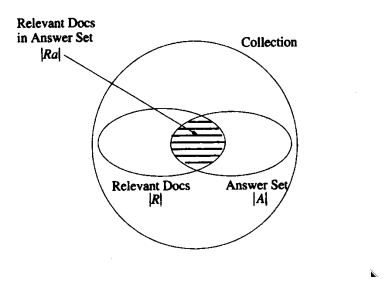
\includegraphics[width=10cm, angle=0]{Figures/Precision-Recall.png}}
	\end{center}
	\caption{Ensemble des documents \citep{modern-ir}}
	\label{fig:precision-recall}
\end{figure}

\subsubsection{Précision}
Le précision (precision en anglais) est la fraction du nombre de documents pertinent par le nombre de documents retournés par le système. En d'autre terme, la fraction des documents retournés qui sont pertinents. La précision calcule alors la performance du système a récupérer seulement les documents pertinents \citep*{evaluation-of-ir-system, ir-on-web,vsm-for-arabic-language}. Le but est de maximiser cette valeur.

\[
	Précision = \frac{\textit{Nombre de documents pertinents}}{\textit{Nombre de documents retournés par le système}} = \frac{|Ra|}{|A|}
\]

\subsubsection{Rappel}
Le rappel (recall en anglais) est la fraction entre le nombre de documents pertinents retournés divisé et le nombre total des documents pertinents. En d'autre terme, c'est la fraction des documents pertinents qui sont retournés par le système. Le rappel permet de savoir comment le système a bien récupérer tous les documents pertinents \citep*{evaluation-of-ir-system, ir-on-web,vsm-for-arabic-language}. Le but est de minimiser cette valeur.

\[
	Précision = \frac{\textit{Nombre de documents pertinents}}{\textit{Nombre de tous les documents pertinents}} = \frac{|Ra|}{|R|}
\]

Il est nécessaire de noter que le rappel n'est efficace dans le cas où la base de données devient large, car le rappel diminue si la base de données augmente. 

\subsection{Exemple de précision et rappel}
Un exemple de calcul de précision et rappel est illustré dans la Figure~\ref{fig:example-prec-rec}.
\begin{figure}[htbp]
	\begin{center}
		\fbox{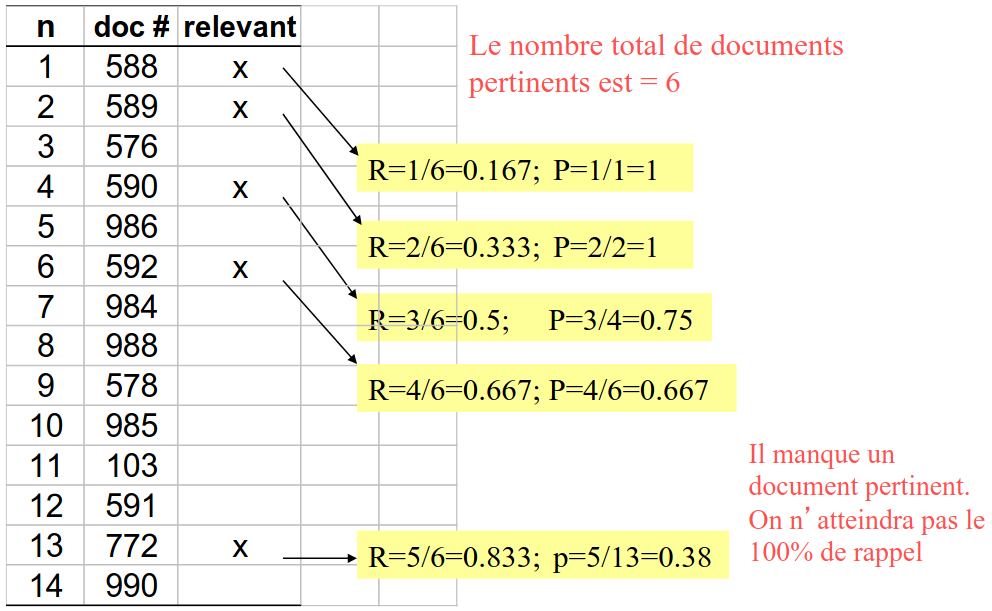
\includegraphics[width=15cm, angle=0]{Figures/SRI/ex-prec-rec.png}}
	\end{center}
	\caption{Exemple de calcule de précision et rappel \citep{evaluation-sri-cours}}
	\label{fig:example-prec-rec}
\end{figure}

Et la courbe (relation) entre la précision et le rappel est illustré dans la Figure~\ref{fig:example-prec-rec-courbe}
\begin{figure}[htbp]
	\begin{center}
		\fbox{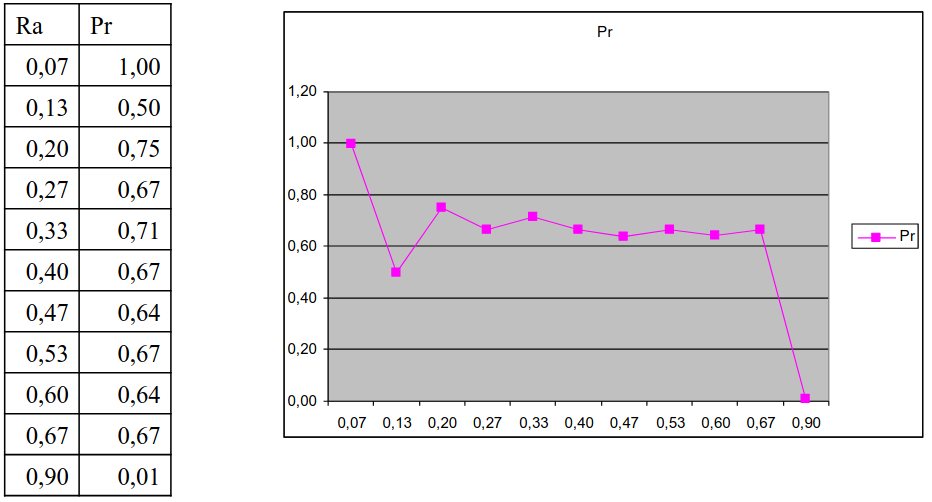
\includegraphics[width=16cm, angle=0]{Figures/SRI/ex-prec-rec-courbe.png}}
	\end{center}
	\caption{Courbe précision-rappel \citep{evaluation-sri-cours}}
	\label{fig:example-prec-rec-courbe}
\end{figure}

\subsection{Problème de précision et le rappel}
(A discuter et a compléter - Modern IR)

\subsection{Moyenne harmonique}
Cette mesure utilise la précision et le rappel.

\[
	F(j) = \frac{2}{\frac{1}{R(j)} + \frac{1}{P(j)}}
\]
\\Où:\\
\textbf{\textit{R (j)}} est le rappel pour le j-ième document.\\
\textbf{\textit{P (j)}} est la précision pour le j-ième document.\\
\textbf{\textit{F (j)}} est la moyenne harmonique

\subsection{Et d'autres mesures}
D'autres mesure de performance sont utilisés comme \textit{accuracy}, \textit{F-measure}, \textit{E-measure}, \textit{x-precision}, etc. Il y a aussi de notion de silence et bruit \citep*{modern-ir, amelioration-ri-approche-semantique}.

\section{Analyse du moteur de recherche existant}
Il y a beaucoup des moteurs de recherche où on peut trouver des thèses malagasy mais dans le cadre de ce mémoire, on va analyser quelques uns qui sont populaire et qui concerne le mieux notre étude.

\subsection{Thèses malgache en ligne}
Thèse malgache en ligne \citep{these-malgache-en-ligne} est un SRI orienté WEB spécialisé pour la recherche des thèses soutenues dans les six universités publiques de Madagascar depuis 2006. Actuellement il regroupe actuellement \textbf{31160} documents, plus précisément des thèses. Ce SRI est hébergé dans le serveur de l'université d'Antananarivo, et est mis en place par les équipes au sein de l'université. Le statistique des documents est dans la figure \ref{fig:statistic-tme}, les résultats de recherche ainsi que la pagination est illustré dans la figure \ref{fig:resultat-tme} et \ref{fig:pagination-tme}.

\begin{figure}[htbp]
	\begin{center}
		\fbox{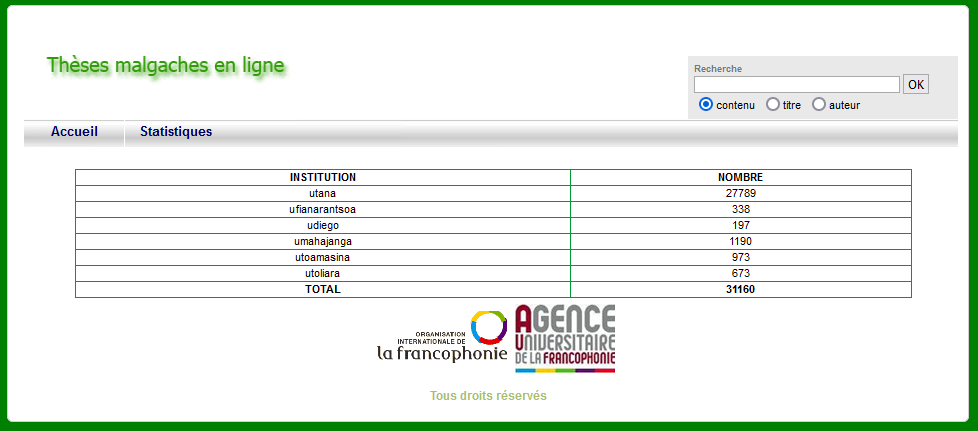
\includegraphics[width=16cm, angle=0]{Figures/SRI/tme-statistics.PNG}}
	\end{center}
	\caption{Statistique des documents \citep{these-malgache-en-ligne}}
	\label{fig:statistic-tme}
\end{figure}

Ce SRI a pour objectif de faciliter les recherches de thèses, généralement d'auteur malagasy afin d'explorer et de mettre en évidence les fruits de recherche malagasy. Ainsi de faciliter l'accès a ces documents pour les enseignants ainsi que pour les étudiants qui cherche des travaux rattachés a son thème.

Ce SRI a un avantage majeur, qui est la rapidité de la recherche. Aussi il y a la possibilité de rechercher par un titre, auteur et contenu, ainsi que la mise en place de système de pagination pour classer les documents plus pertinents dans la première page. Ce SRI classe les résultats suivant l'ordre de pertinence décroissant. L'interface utilisateur est très simple ce qui implique que le chargement de la page est rapide.

Ce Système a quelques lacunes malgré ses avantages. La première problème qui peut être remédié est l'insuffisance de nombre des documents stockés, car vu le nombre d'étudiants ayant soutenu dans les six universités publiques de Madagascar, c'est pas suffisant. La deuxième, les documents sont limités pour les établissements publiques, alors qu'il pourra être intéressant d'inclure les documents des établissement privés. La troisième c'est qu'il y a pas de système de catégorisation des documents. Et d'autres problèmes comme le nombre de documents retournés sont nombreux qui implique souvent beaucoup de pagination des résultats (pas de limite de pertinence), il est impossible de voir la résumé d'un document particulier ou afficher une aperçu du document, et finalement il y a pas de notion de sécurité de document c'est a dire tous les documents sont exposés publiquement en tant qu'utilisateur anonyme.

\begin{figure}[htbp]
	\begin{center}
		\fbox{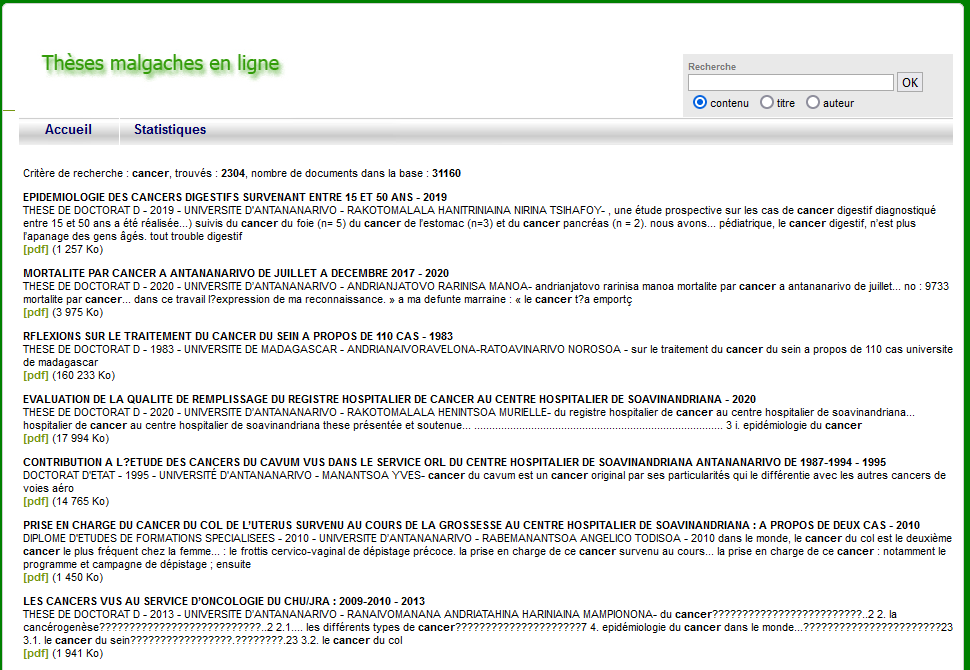
\includegraphics[width=16cm, angle=0]{Figures/SRI/tme-results.PNG}}
	\end{center}
	\caption{Resultat de recherche \citep{these-malgache-en-ligne}}
	\label{fig:resultat-tme}
\end{figure}

\begin{figure}[htbp]
	\begin{center}
		\fbox{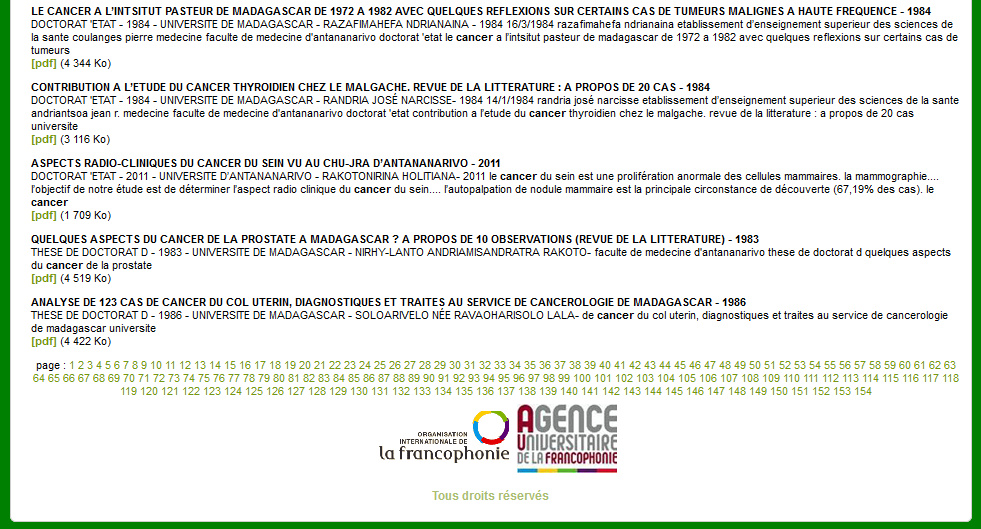
\includegraphics[width=16cm, angle=0]{Figures/SRI/tme-pagination.PNG}}
	\end{center}
	\caption{Pagination \citep{these-malgache-en-ligne}}
	\label{fig:pagination-tme}
\end{figure}

\subsection{Bibliothèques universitaire en ligne}
Les bibliothèques universitaire en ligne n'est plus ni moins qu'une version numérique des bibliothèques. Chaque université publique de Madagascar possède un. En général, c'est pas un SRI complet mais juste une liste des documents disponibles avec un simple recherche généralement sur le titre ou auteur. 

L'objectif est d'exposer des documents pour faciliter l'accès aux étudiants, enseignants ou des personnes voulant accéder a des ressources. Mais en général, ce système fonctionne très bien avec un recherche simple dans le cas des livres par exemple, mas s'avère compliqué pour des recherches avancés. Ainsi les documents sont incomplètes. 

Dans le cadre de recherche des thèses malagasy, ce système est moins efficace que Thèse malgache en ligne.

\subsection{Google Scholar, theses.fr et d'autres}
Les géants du moteurs de recherche académique tel que google scholar, Mémoire online, HAL, et d'autres peuvent bien être utilisé pour rechercher des thèses malagasy. Ces systèmes sont performants, puissant en terme d'algorithme utilisés, et stock une grande volume des documents. Certains système propose d’aperçu du document, exportation des bibliographie, liste des articles connexes ainsi qu'un système de sécurité et d'authentification. Il est aussi possible de faire une filtre par année ou par catégorie.

Malgré tous ces atouts, c'est pas suffisant pour les travaux de recherches malagasy. Ces moteurs n'arrivent pas a indexer beaucoup des documents (thèses) malagasy. Par exemple, dans thèses.fr, il y a seulement 41 thèses en cotutelle pour l'université d'Antananarivo \citep{these-fr}. Alors pour rechercher des travaux de recherche malagasy dans ces moteurs est un véritable défi.

\section{Conclusion}
En résumé, un Système de Recherche d'Information ou Moteur de Recherche est un système actuellement indissociable de la vie quotidienne, académique, personnel et professionnel. Il a pour but de satisfaire le besoin d'information de l'utilisateur en utilisant des algorithmes et des traitements particulières sur les documents et la requêtes. Un SRI doit passer certains test avant d'être finalement implémenté pour l'utilisation finale. Ces testes sera réalisé pas des experts du domaine, et en utilisant des corpus de test (collection de test) pour pouvoir déterminer la pertinence et la performance du SRI. Il y a actuellement beaucoup des moteurs de recherche, certains sont spécialisés dans un domaine spécifique, mais on a analysé justement quelques un qui est important dans le cadre de ce devoir.


\section{Traitement de Langage Naturel (TLN)}
\subsection{Introduction}
Le Traitement de Langage Naturel (Natural Langage Processing) est une approche pour analyse des textes qui est basé sur les théories et la téchnologies. C'est un domaine très répandu actuellement dans la recherche et developpement \citep{natural-language-processing}. La NLP est utilisé dans la recherche d'information, traduction des textes, traduction des voix, système de question reponse ainsi que diverses domaines.

\begin{definition}[NLP]
    Natural Language Processing (NLP) est un discipline qui combine la linguistique, l'informatique et l'intelligence artificielle pour analyser et etudier les intéractions entre uns système informatique et une langage naturel humain. La Recherche d'Information est parmi l'une de tâche du NLP \citep{art-nlp}.
\end{definition}

\begin{definition}[NLP]
    Selon \citeauthor{natural-language-processing}, un NLP est un ensemble des téchniques informatiques théoriques motivés pour analyser et represeter naturellement des textes (un langage quelconque) en passant par un ou plusieurs niveaux d'analyse linguistique dans le but de parvenir a traiter le langage humain dans un étendu de tâches ou applications \citep{natural-language-processing}.
\end{definition}

L'analyse de langage, porte a connaitre la structure de langage tel que les mots, les significations, combinaison des mots, ainsi que la contribution des mots au sense de la phrase. Et aussi d'analyser le fonctionnemet du monde et le raisonnement de l'humanité dans le monde \citep{automatic-nlp}.

Le domaine de TLN a quelques divisions tel que:
\begin{itemize}
    \item \textbf{NLP}: production de representation significatif. Equivalent du rôle de lecteur et ecouteur.
    \item \textbf{NLG}: production de langage a partir d'une representation. Equivalent du role d'auteur et interlocuteur.
    \item \textbf{Language Understanding}: Termine avec un langage orale.
    \item \textbf{Speech Understanding}: Demarre avec un langage orale. Permet de savoir comment un langage orale va se traduire en texte.
\end{itemize}

Le domaine NL par rapport a l'intelligence artificielle est illustré dans la figure \ref{nlp-ref-ai}.

\begin{figure}[htbp]
    \begin{center}
        \fbox{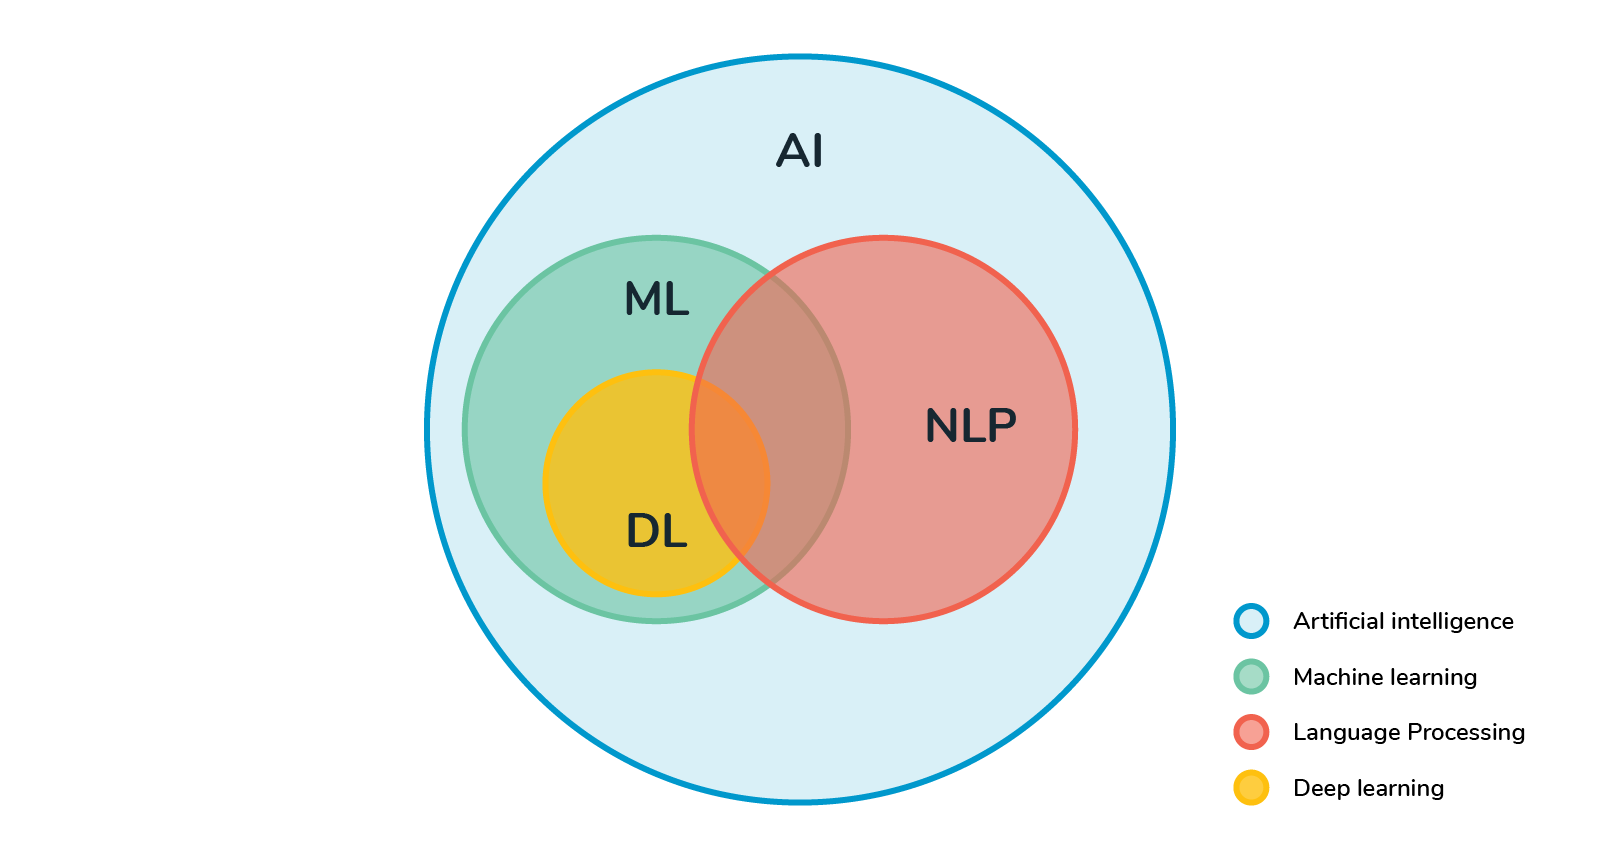
\includegraphics[width=13cm, angle=0]{Figures/NLP/nlp-ref-ai.png}}
        \caption{Position du TLN par rapport a l'IA \citep{devopedia-nlp}}
    \end{center}
    \label{nlp-ref-ai}
\end{figure}

Certains notion qu'on abordera ici sont déja presenté dans la section (Processus de recherche d'information), donc certains notions ne seront pas détaillés.

\subsection{Un peu d'histoire}
Cette briève historique est tiré de l'ouvrage de \citeauthor{natural-language-processing} \citep{natural-language-processing}. La recherche en Traitement de Langage Natures trouve ses origines dans les années 1940. Le MT (Machine Translation) est la prémière application en NLP qui est une application d'ordinateur. En 1946, Weaver et Booth demarre l'une de projet recent de MT, encore sur la traduction basé sur l'expertise de voler le code d'énemie durant la deuxième guerre mondiale. Ce projet a suggerré l'utilisation de la cryptographie et de la théorie de l'information pour le traduction de langage. Puis la recherche sont devenu varié dans les institutions en Etats-Unis d'Amérique (USA).

En 1957, Chomsky a publié Syntactic Structure, qui introduit l'idée de grammaire génerative pour remedier aux problèmes rencontré dans les années anérieurs tel que l'ambiguité syntaxique, \dots Une autre domaine de NLP commence aussi a emerger, qui est la reconnaissance vocale.

La communauté de Traitement de langage et la communauté vocale (Speech community) était divisé alors en deux camps: d'une part la communauté de traitement de langage dominé par la théorie perspective de grammaire generative et hostile en methode statistique; et d'autre part la communauté vocal (SC) dominé par la théorie statistique de l'information et hostile en théorie linguistique.

En 1950, l'homme pense que la meilleur qualité totalement automatique peut produire des resultats indiscernable de la translation huamine, et qu'un tel système peut être opérationnel dans quelques années.

Enfin, la NLP a connu beaucoup d'évolution ainsi des nombreuses lacunes. A partir des années 1980, la NLP a evolué beaucoup plus vite par la dispositions des ressources computationel ainsi que des ordinateurs performants.

\subsection{Les niveaux de langage}
Un langage comporte géneralement cinq niveaux ou étape de traitement \citep*{automatic-nlp, handbook-nlp} et qui est illustré dans la figure \ref{nlp-stage}:
\begin{itemize}
    \item \textbf{Phonétique et phonologie}: la liaison des mots et des phrases au son qui les réalisent a l'oral. Cette niveau n'est past utile dans le traitement de langage textuelle.
    \item \textbf{Morphologie}: la façon dont les mots sont construits, et de connaitre leurs rôles dans la phrase.
    \item \textbf{Syntaxe}: la façon dont les mots se combinent pour former des \textit{syntagmes}, puis des proposition et enfin des phrases correctes. Un \textbf{syntagmes} est un unité syntaxique intermédiaire entre le mot et la prase, et comprenant un seul noyau et souvent des compléments.
    \item \textbf{Sémantique}: la façon dont les mots font du sens lorsqu'ils sont insérés dans une phrase indépendamment du contexte.
    \item \textbf{Pragmatique}: la façon d'interpreter les phrases selon leur contexte d'énonciation comme l'interlocuteur, phrase précedente, connaissance commune du monde, \dots
\end{itemize}

\begin{figure}[htbp]
    \begin{center}
        \fbox{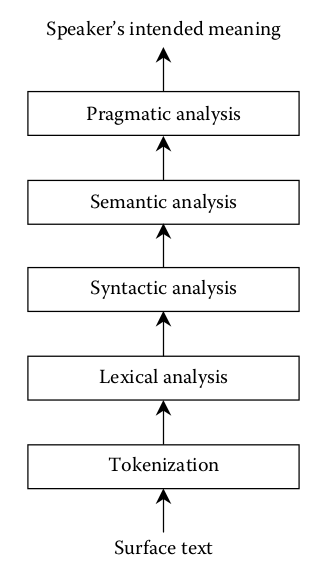
\includegraphics[width=8cm, angle=0]{Figures/NLP/nlp-stage.png}}
        \caption{Etape d'analyse de texte dans NLP \citep{handbook-nlp}}
    \end{center}
    \label{nlp-stage}
\end{figure}

\subsection{Phonologie}
La phonologie interprète le langage parlé (son de parole) dans un mot \citep{natural-language-processing}. Il y a trois règles tel que:
\begin{itemize}
    \item \textbf{Règle phonétique}: pour les sons dans les mots.
    \item \textbf{Règle phonémique}: pour les variations de prononciation quand les mots son prononcé ensemble.
    \item \textbf{Règle prosodique}: pour la variation d'un stresse et d'intonation dans un phrase.
\end{itemize}

\subsection{Morphologie}
La morphologie est l'étude de la forme des mots tel que leur \textit{fléxion}: indication de cas, genre, nombre, mode et temps; leur \textit{derivation}: préfixes, suffixes et infixes; leur \textit{composition}: mots composés. C'est aussi une analyse morphosyntaxique, qui analyse des règles de combinaison des morphèmes selon la configuration syntaxique de l'énnoncé. La morphologie consiste a segmenter des textes en unités élémentaire qu'on appelle \textit{tokenisation} et à determiner les différentes caractéristiques de ces unités \citep{automatic-nlp,natural-language-processing}.

Un humain est capable de faire ce traitement pour comprendre le sens, vu que chaque sens des morphèmes ne change pas dans tous les mots, et idem pour un système NLP qui consiste a reconnaitre le sens porté par chaque morphème pour representer le sens \citep{natural-language-processing}.

\begin{definition}[Lemme]
    On appelle \textit{lemme} la racine d’un mot, sans ses marques d’accord, de conjugaison, de cas. L'entrée d'un dictionnaire est généralement un lemme. Le lemme est necessaire dans toute analyse sémantique. \citep{automatic-nlp}
\end{definition}

\begin{definition}[Flexion]
    Les \textit{flexions} sont les modifications opérées sur le lemme pour distinguer les formes de conjugaison (personne, temps, mode, voix – flexion verbale) ou le genre, le nombre et le cas (flexion nominale).L’opération qui consiste à retrouver ces informations est la \textit{lemmatisation}, ou souvent appellé \textit{racinisation (stemming)} \citep{automatic-nlp}.
\end{definition}

\begin{definition}[Morphème]
    On appelle \textit{morphème} le plus pétit unité ou unité minimale de sens \citep{natural-language-processing}. Par exemple, le mot pretraitement est composé de trois morphèmes tel que le prefix \textbf{pre}, la racine \textbf{traite} et la suffixe \textbf{ment}.
\end{definition}

Cette étape est une parite essentiel du NLP, qui est necessaire pour definir les caractères, mots et phrases dans un document. Cette rélève un défi tel que la résolution des ambiguités dans le langage naturel ainsi que de convertir des fichiers textes dans un séquence de texte bien défini eavec un sens. Cette étape peut être divisé en deux parties: \textit{Triage de document (Document Triage)} et \textit{Ségmentation de texte (Text Segmentation)} \citep{handbook-nlp}.

\subsubsection{Triage de document}
Le triage de document c'est l'action de convertir un ensemble des fichiers en documents textuelles bien définie. Il se decompose en trois étapes tel que:
\begin{enumerate}
    \item \textbf{Identification d'encodage de caractère (Character Encoding Identificator)}: permet d'identifier l'encodage de caractère utilisé dans le fichier a convertir, par exemple si le fichier utilise l'encodage UTF-8 ou ISO ou autres.
    \item \textbf{Identification de langage (Language Identification)}: permet de determiner dans quelle langue le fichier est écrit (Français, Anglais, etc.).
    \item \textbf{Sectionnement de texte (Text Sectionning)}: permet d'identifier le conténu textuel du fichier pour pouvoir le convertir een document textuel bien défini.
\end{enumerate}

\subsubsection{Segmentation de texte}
La segmentation de texte est un étape cruciale et complexe dans la Traitement de Langage Naturel. Il consiste a convertir un document textuel bien déifnie en composant des mots et des phrases \citep{handbook-nlp}. C'est aussi la transformation d'un alignement d'un caractère en une unité élementaire souvent des mots et phrase \citep{automatic-nlp}. Généralement, il y a trois étapes tel que la \textit{ségmentation de mot (Word segmentation)}, la \textit{normalisation de texte (Text Normalization)} et la \textit{ségmentation de phrase (Sentnce Segmentation)}.

Pour la segmentation de texte, il faut éfinir une liste de caractères délimiteur pour pouvoir segmenter le texte (espace, ponctuation, apostrophe). Pour les langages dont l'espace n'est pas un délimiteur comme la langue chinoise par exemple, cette segmentation est plus complexe \citep{handbook-nlp}. Et même avec la langue qui a comme délimiteur les trois cités ci-dessus, il est encore compliqué de separé les mots, car l'apostrophe peut être utilisé dans un seul mot comme \textit{aujourd'hui}, aussi un unité élémentaire peut conténir des éspaces comme \textit{pomme de terre} \citep{automatic-nlp}.

En pratique le système de segmentation du texte utilise une liste de sépatateurs par defaut, a laquelle ils ajoutent des connaissances lexicales et morphosyntaxiques pour traiter les cas ambigus. Chaque lange possède ses propres connqissances léxicales.

\subsubsubsection*{Segmentation de mot}
La segmentation de mot c'est l'action couper un sequence des caractères en texte par la localisation de delimiteur de mot (Word boundaries) pour pouvoir être utilisé dans la traitement linguistique. Un délimiteur permet de définir le point où un mot est terminé et qu'un autre commence. Les mots obténues sont appelées des \textit{tokens}, et la façon d'obtenir ces tokens est la \textit{tokenisation ou tokenization en anglais}. \citep{handbook-nlp}

Pour les langages delimité par un espace (space-delimited), souvent des langages européennes, les mots sont séparés par des espaces. Tandis que pour des langages qui ne sont pas delimités par un espace comme le Chinois et le Thai, il n'y a pas d'indication sur le delimiteur \citep{handbook-nlp}. Dans le cadre de ce devoir, on travaillera sur des langages qui a comme délimiteur espace.

Dans un langage délimité par un espace, les ponctuations sont souvent traité comme des tokens separés, mais qui varie d'un langage a un autre. Masi souvent pose de problèmes comme des abbréviation, les quotes et les appostrophes. \citep{handbook-nlp}

\subsubsubsection*{Normalisation de texte}
La normalisation de texte permet de fusionner les différentes formes de token en une forme canonique normalisé par exemple Mr et Monsieur. Cette normalisation permet aussi de normaliser des dates, des heures, des formats monétaires et d'autre informations numériques. Par exemple, les trois tokens écrit \$300 peut être prononcé comme \og{trois cent dollars} \fg{} et la normalisation de texte peut convertir le token original en token desiré. \citep{handbook-nlp}

\subsubsubsection*{Segmentation de phrase}
C'est de determiner comment le texte doit être divisé en phrase pour un traitement plus avancé. En identiiant les délimiteurs de phrase (souvent un point pour la langue delimité par un espace). Souvent la segmentation de phrase est referencé comme \textit{detection de dilimiteur de phrase} ou \textit{desambiguition de délimiteur de phrase} ou encore \textit{reconnaissance de délimiteur de phrase} \citep{handbook-nlp}.

\subsubsection{Catégories grammaticales}
Les catégories grammaticales est une information morphosyntaxique importante. Ces catégories sont souvent des noms, verbe, adjectif, mais qui varie selon le système. Par exemple \textit{Penn Treebank} contient 45 catégories. Sur la figure \ref{categorie-grammaticale} un exemple de catégorie grammaticale pour la phrase \textit{\og Qui veut noyer son chien l’accuse de la rage \fg{}}, et qui illustre aussi la problème d'ambiguité pour cette phrase. En général 25\% du lexique est de forme ambigus pour la langue française. Et un exemple de description morphosyntaxique illustré dans la figure \ref{exemple-desc-morphosyntaxique}.

\begin{figure}[htbp]
    \begin{center}
        \fbox{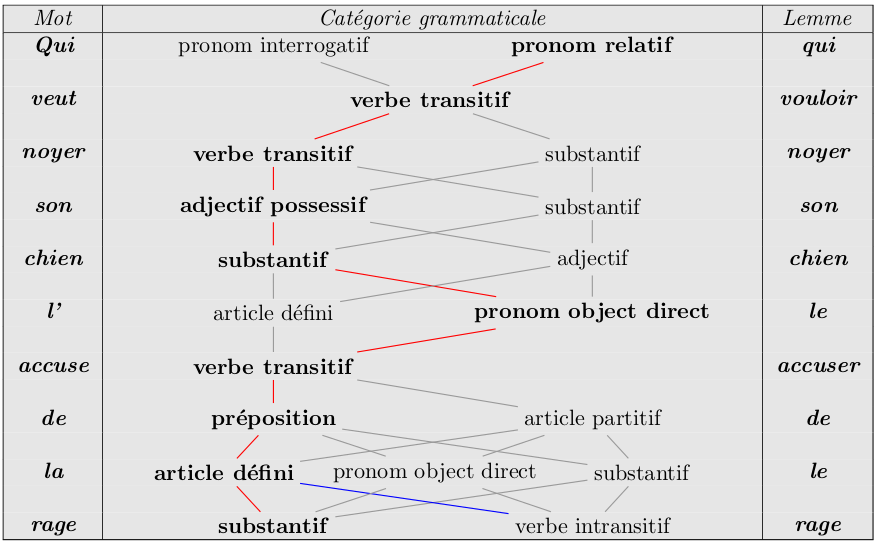
\includegraphics[width=15cm, angle=0]{Figures/NLP/classe-grammatical.png}}
        \caption{Catégorie grammaticale \citep{handbook-nlp}}
    \end{center}
    \label{categorie-grammaticale}
\end{figure}

\begin{figure}[htbp]
    \begin{center}
        \fbox{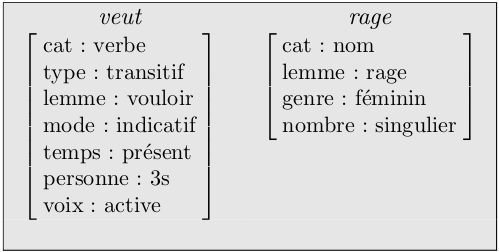
\includegraphics[width=10cm, angle=0]{Figures/NLP/description-morphosyntaxique.png}}
        \caption{Description morphosyntaxique \citep{handbook-nlp}}
    \end{center}
    \label{exemple-desc-morphosyntaxique}
\end{figure}

\subsection{Analyse lexicale}
Un humain ou un Système NLP interptète le sens de chaque mot individuellement. L'analyse lexicale permet alors de determiner le sens de chaque mot individuellement. Le but est de contribuer au comprehension de niveau de mot par une affectation de tag \textit{part-of-speech} pour chaque mot. Un mot qui a un sens possible peut être remplacé par un representation semantique de ce sens \citep{natural-language-processing}.

Un analyse lexicale utilise un lexicon, qui est determiné et choisi par le système NLP. Un lexicon peut être \textbf{simple} c'est à dire des mots et ses \textit{pos} ou peut être \textbf{complexe} et contient l'information de classe sémantique des mots \citep{natural-language-processing}.

\subsection{Syntaxe}
La syntaxe décrit comment les lemmes ou fléxions sont ordonnées pour créer des constituants, composant aux-mêmes des phrases. Souvent, l'analyse syntaxique est representé de façon hierarchique. Dans l'analyse syntaxique, on travaille avec les mots, les phrases, ainsi que l'étape de la formation du mots a la phrase \citep{automatic-nlp}. L'analyse syntaxique est une analyse complexe avec différentes niveaux, les détails ne seront pas traité dans ce dévoir, mais présent dans la section 3 \citep{automatic-nlp} et section A DETERMINER (Handbook NLP).

L'analyse syntaxique selon (Auteur NLP tout court), se focalise sur l'analyse des mots dans une phrase, pour decouvrir la structure grammaricale de la phrase, qui necessite l'utilisation de la grammaire et un parseur. Dans l'analye syntaxique, l'ordre et le depenance des mots contribue au sens: par exemple, la phrase \textit{\og Le chat attaque le chien \fg{}} et la phrase \textit{\og Le chien attaque le chat \fg{}} ont un sens différent car ses termes de sytaxe est différent, pourtant ils sont composé des mêmes mots \citep{natural-language-processing}.

\subsubsection{Analyse syperficielle}
\citep{automatic-nlp} Le but de l'analyse superficielle ou partielle, est de reconnaitre les syntagmes simples, non récursif d'un énoncé sans lier les uns aux autres; d'obtenir des résultats moins riches mais plus sûr et plus rapide. Cette approche s'oppose a l'analyse profonde ou complète qui cherche a regrouper chaque phrase dans une unique representation.

\textbf{Cass} est un exemple de d'analyseur partielle efficace, qui consiste en une cascade d'automates à états finis.

\subsubsection{Analyse en dépendance}
L’analyse syntaxique en dépendance diffère surtout de l’analyse en constituants (comme les règles hors-contexte) par le mode de représentation. Les deux approches n’ont pas de différence au niveau de leur couverture ou de leur expressivité (A reformuler). L'idée est de relier les mots et non les constituants \citep{automatic-nlp}.

Un exemple de grammaire de dépendance est la \emph{Link Grammar} qui définit la lexique et les contraintes d'attachement, comme illustré dans la figure \ref{link-grammar} et \ref{link-grammar-syntax}

\begin{figure}[htbp]
    \begin{center}
        \fbox{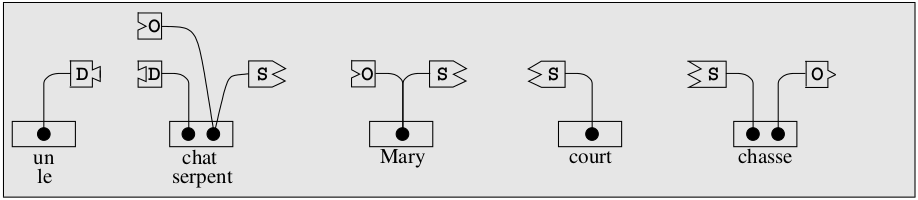
\includegraphics[width=13cm, angle=0]{Figures/NLP/lexic-link-grammar.png}}
        \caption{Exemple de définition de la lexique \emph{Link Grammar} \citep{automatic-nlp}}
    \end{center}
    \label{link-grammar}
\end{figure}

\begin{figure}[htbp]
    \begin{center}
        \fbox{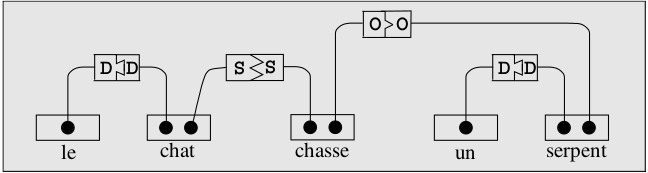
\includegraphics[width=13cm, angle=0]{Figures/NLP/syntax-link-grammar.png}}
        \caption{Exemple d'analyse syntaxique avec \emph{Link Grammar} \citep{automatic-nlp}}
    \end{center}
    \label{link-grammar-syntax}
\end{figure}

\subsection{Sémantique}
Un approche sémantique peut être utilisé pour reduire les ambiguités syntaxiques, a mieux cibler des contextes (en RI par exemple), mais son but finale est de représenter formellement l’information véhiculée par un énoncé et éventuellement d’en inférer de nouvelles connaissances ou une réponse à la question posée dans le cas où l'énoncé est une question \citep{automatic-nlp}. Il a pour but d'associer a un sequence de mots une répresentation interne de son sens, tout en prenant compte l'utilisation futures des resultats obtenues.

Selon beaucoup des personnes, c'est dans le niveau sémantique qu'on determine la signification, pourtant tous les niveaux contribuent au signification. La sémantique determine alors la signification possible d'une phrase en se concentrant sur l'interaction parmi les significations de niveau des mots dans une phrase, avec la possibilité de desambiguition sémantique des mots aux multiple sens. Par exemple si on prend le mot \textbf{pile}, ca peut être un pile pour alimenter un appareil electronique, ou ca peut être un structure dans un langage de programmation informatique.

Selon \citeauthor{automatic-nlp}, il y a quatres méthodes:
\begin{itemize}
    \item \textbf{L'analyse profonde}: permet d'obtenir une representation complète de l'enoncé
    \item \textbf{Interpretation sémantique grammaticales}: qui s'appuie sur une analyse syntaxique totale
    \item \textbf{Grammaires sémantiques}: qui modelisent les données spécifiques
    \item \textbf{Patrons sémantique}: qui detectent les informations prédefinies dans un texte
\end{itemize}

On distingue deux types de sémantique tel que la \textit{sémantique grammaticale} qui se charge a construire un sens de l'énoncé globale, et la \textit{sémantique lexical} qui étudie la participation des mots a ce sens et tous les ambiguités qu'ils provoquent.

\citeauthor{amelioration-ri-approche-semantique,approche-semantique} \citep{amelioration-ri-approche-semantique,approche-semantique} ont chacun developpé un moteur de recherche basé sur cette notion de sémantique pour ameliorer la qualité de recherche, et analyser les ambiguités dans un terme de recherche des utilisateurs.

\subsubsection*{Quelques rélations importantes entre les mots}
Il y a des relations importantes entre les mots \citep{automatic-nlp} qui est necessaire en analyse sémantique tel que:
\begin{itemize}
    \item \textbf{Polysémie et l'homonymie}: propriété de certains formes graphiques (signifiants) de renvoyer à plusieurs sens (signifié). Par exemple, le mot \textit{bureau}.
    \item \textbf{Synonmie}: lien entre deux mots ayant la même sens.
    \item \textbf{Hyponymie}: relation d'inclusion entre deux mots dont l'un (hyponymie) est plus spécifique que l'autre (hyperonyme). Par exemple le mot \textit{gorille} est un hyponimie du mot \textit{quadrimane}, le mot \textit{fleur} est un hyperonymie du mot \textit{tulipe}.
    \item \textbf{Méronymie et holonymie}: relation de partie a tout. Par exemple, une serrure est une partie d'une cage (meronymie), un batiment contient une pièce (holonymie).
\end{itemize}

Ces relations existant entre les mots sont repertoriés dans des base informatiques dont le plus utilisés est \textbf{WORDNet}.

\subsection{Pragmatique}
\citeauthor{natural-language-processing} cite un niveau supplémentaire entre la sémantique et la pragmatique, c'est le \textbf{discours} qui travaille sur un texte plus longue qu'une phrase et interprète le sens en connectant tous les phrases. Il y a deux types de traitement de discours tel que: l'\textit{Anaphora} et le \textit{Discours/text structure recognition}.

Tandis que l'analyse pragmatique sert dans un sitiation bien spécifique, utilise de contexte qui dépasse le contenu de comprehension de texte \citep{natural-language-processing}. En d'autres termes, regroupe un grand nombre de domaine qui englobent tous les problèmes qui ne pouvant être traités avec la syntaxe et la sémantique \citep{automatic-nlp}. Cette analyse necessite l'utilisation des connaissances extra-linguistiques sur le contexte et du discours. Pour cette raison que les application pratiques sont rares, pourtant il y a quelques uns \citep{automatic-nlp} comme la \textit{diéctique}, l'\textit{implicateurs conversationnelle} et la \textit{presupposition}.

\subsection{Approche du TLN}
Il y a généralement trois approche dans la Traitement de Langage Naturel, tel que l'\textit{approche symbolique}, l'\textit{approche statistique} et l'\textit{approche connexionniste}.

\subsubsection{Approche symbolique}
Cette approche a coexisté avec l'approche statistique le jour après la naissance de ce domaine. Elle fait une analyse profonde des phénomèmes linguistiques, et qui est basé sur la representation explicite des faits a propos d'un langage a travers une connaissance bien compris. Cette approche a été trouvé dans un système basé sur des règles (ensemble des règles, moteur d'inférence et un espace de travail); ou logique: structure sans forme de proposition logique.

L'approche symbolique est appliqué dans diverses domaines de recherche comme l'\textit{extraction d'information}, la \textit{catégorisarion de texte}, \textit{resolution d'ambiguité}, et l'\textit{acquisition lexicale}.

\subsubsection{Approche statistique}
Cette approche, souvent utilisé un large volume de texte (corpora), emploi des techniques mathématiques variés pour developper des modèles approximatif generalisé de phénomène liguistique. Cette approche utilise des données observables comme source primaire d'évidence. Le modèle statistique souvent utilisé est le \emph{HMM} ou \emph{Hidden Markov Model}.

L'approche statistique est appliqué dans la \textit{reconnaissance vocale}, \textit{acquisition lexicale}, \textit{parsing}, \textit{part-of-speech tagging}, \textit{machine de translation statistique}, \textit{collocations}, \textit{apprentissage statistique de grammaire}.

\subsubsection{Approche connexionniste}
Cette approche est apparu dans les années 1960, est comme l'approche statistique qui developpe des modèles generalisés depuis l'exemple de phénomène linguistique. Elle combine l'apprentissage statistique avec différentes \emph{théories de representation} qui permet la transformation, l'inférence et la manipulation de formule logique.

Certains modèles de l'approche connexionniste s'appelle \textbf{modèle localiste} qui peut faire des tâches comme \emph{desambiguition de sens de mot}, \emph{generation de langage}, et \emph{inference limité}; et \textbf{modèle distribué} qui est utilisé pour les tâches comme la \emph{parsing des syntaxes (syntactic parsing)}, \emph{translation dans un domaine limité ou spécifique} et \emph{recherche associative}.

\subsection{Application de TLN}
La Traitement de Langage Natuel s'applique dans diverses domaines de recherche que ce soit textuelle ou sonores.

\subsubsection*{La Recherche d'Information (RI)}
Dans la recherche d'information, on travaille sur des textes, ce qui impique que certains implémentation utilise le NLP. Cette application utilise souvent l'approche statistique \citep{natural-language-processing}. Le TLN est généralement utilisé dans le niveau traitement morphologique.

Elle analyse la variation morphologique des mots ou \emph{stemming}, mais aussi la variation syntaxique (etude des syntagmes nominaux) ainsi que la variation sémantiques: relation liant des lemmes différents mais identiquement proches et la multitude de sens qui peut prendre une forme graphique donnée (polysémie, homonymie) \citep{automatic-nlp}.

\subsubsubsection*{Stemming}
\citep{automatic-nlp} La plus courante utilise une approximation des phénomènes linguistiques d'une langue donnée, comme les mécanismes habituels de conjugaison, d'accord ou de genre et en nombre, ou sa derivarion et tente de supprimer les suffixes rout en regroupant les différentes allomorphes (variante graphique d'une même racine).

Lealgorithme le plus utilisé est celle de \emph{Lovins} et \emph{Porter} pour la langue anglaise et \emph{Jacques Savoy} pour la langue française.

\subsubsection*{L'Extraction d'Information (EI)}
Ce domaine d'application est plus recente, qui se base sur la reconnaissance, marquage (tagging), et extraction dans un representation structurés, certains éléments clés d'information, par exemple: personne, companie, localisation, organisation, d'un large collection de texte \citep{automatic-nlp}.

\subsubsection*{Et d'autres applications}
Et d'autres dommaines d'applications, comme la machine de traduction (Machine Translation), système de dialogue, système de question-reponse, système de resumé (summarization).

\subsection{Conclusion}
En conclusion, la TLN est l'un de domaine interessant, et contribue a beaucoup des recherches dans la domaine de l'informatique. Il est aussi necessaire dans la recherche d'information. Elle se divise en deux principale branches qui est le traitement de langage ecrite et le traitement de langage orale. Elle propose différentes approches eet méthodes ainsi que différentes algorithmes pour faire des traitements. Elle est utilisés dans différentes domaines et qui est devenue indissociable de l'intelligence artificielle.

\chapter{Modèle vectoriel}
\section{Introduction}
Le modèle vectoriel (Vector Space Model) est l'une de modèle le plus utilisé en recherche d'information, que ce soit textuel \Citep{sarch-engine-vsm} ou multimédia \citep{vsm-images}. Ce modèle est apparu lorsque la pondération binaire est limitant, et que l'appariement partielle n'est pas possible, en introduisant la pondération non binaire et un appaiement partielle \citep{modern-ir}.

Le principe de ce modèle vectoriel modélise la requête et des documents sous forme d'un vecteur, ponderer les termes dans ce vecteur avec des méthodes de pondération comme le \emph{TF-IDF}, et calcule ensuite la distance euclidienne entre les vecteurs documents et la vecteur requête pour determiner la pertinence \citep{ir-on-web}. Un score de similarité est alors calculé pour pouvoir classer les documents jugés pertinent par le système. La representation du document et la requête est illustré dans la Figure~\ref{fig:vector-model} dans la section \ref{sec:vsm-model}.

\begin{definition}[Modèle Véctoriel]
    On note $w_{ij}$ le poids positif et non binaire, du terme i dans le document j qui est associé avec un pair $(k_{i}, d_{j})$ et $w_{iq}$ le poids du terme i dans la requête $q$. La requête est définie par le vecteur: $ \vec{q} = (w_{1q}, w_{2q}, \dots, w_{tq}) $ où $t$ le nombre total des termes d'indexation dans le système. Un document $d_{j}$ est présenté par le vecteur: $ \vec{d_{j}} = (w_{1j}, w_{2j}, \dots, w_{tj}) $.

    La calcul de similarité entre ces deux vecteurs se traduit par la formule:
    \[
        Sim(\vec{d}, \vec{q}) = \frac{\vec{d_{j}} \cdot \vec{q}}{ |\vec{d_{j}}| \times |\vec{q}| } \\
        = \frac{\sum_{i=1}^{t} w_{i,j} \times w_{i,q}}{\sqrt{\sum_{i=1}^{t} (w_{i,j})^2} \times \sqrt{\sum_{i=1}^{t} (w_{i,q})^2}}
    \]

    Avec $ |\vec{d_{j}}| $ et $ |\vec{q}| $ norme du vecteur document et de la vecteur requête.
\end{definition}

Dans le cadre de ce mémoire, c'est cette modèle qu'on utilisera, et on l'ppliquera sur des documents PDF ou WORD.

\section{Problème de classification}
Ce problème est illustré et analyser dans \citep{modern-ir}. L'étude de Salton définit la problème de RI comme un problème de classification. Notons une collection de document \emph{C} et que la requête de l'utilisateur est une vague representation de l'ensemble des documents \emph{A}. Le problème est donc de determiner quelle cocuments appartient a l'ensemble A, qui est un problème de classification.

Dans un problème de classification, il y a deux problème: la prémière consiste a determiner les fonctionnalités qui décrit le mieux les objets dans la collection \emph{A}; et la seconde consite a determiner les fonctionnalités qui distingue les objets dans collection \emph{A} pour les autres objets provenant de la collection \emph{C}. La prémière fonctionnalité produit la quantification \emph{intra-clustering} tandis que la seconde fonctionnalité produit la quantification \emph{inter-clustering}.

Dans le modèle vectoriel, la similarité \emph{intra-clustering} est quantifié par la mesure de la frequende du terme $k_{i}$ dans le document $d_{j}$. Cette facteur est souvent appellé facteur \emph{tf} ou \emph{term frequency}, qui décrit la caratérisation intra-document. D'autre part, la similarité \emph{inter-clustering} est quantifié par la mésure de l'inverse du fréquence du terme $k_{i}$ parmi les documents dans la collection. Cette facteur est souvent appellé facteur \emph{idf} ou \emph{inverse document frequency}

Pour avoir un meilleur classification des documents, il faut balancer ces deux mesures.

\section{Méthodes de pondération des termes}
Cette facteur est permet de calculer la frequence d'un terme dans un document \ref{sec:mesure-similarite}.

\begin{definition}
    Cette définition est tiré de \citetitle{modern-ir} \Citep{modern-ir}. Notons \emph{N} le nombre total des documents dans le système et $n_{i}$ le nombre de documents contenant le terme $k_{i}$. Notons $freq_{i,j}$ la fréquence du terme $k_{i}$ dans le document $d_{j}$ (le nombre de dois où le terme $k_{i}$ est mentionné dans le texte du document $d_{j}$). Alors la frequence normalisé $f_{i,j}$ du terme $k_{i}$ dans le document $d_{j}$ est donné par
    \[
        f_{i,j} = \frac{freq_{i,j}}{\max_{l} freq_{i,j}}
    \]

    où le maximum est calculé a travers les termes qui sont mentionné dans le texte du document $d_{j}$. Si le terme $k_{i}$ n'appartient pas au document $d_{j}$ alors $f_{i,j} = 0$. D'autre part, notons $idf_{i}$ l'\emph{inverse document frequency} pour le terme $k_{i}$, qui est donné par
    \[
        idf_{i} = \log{\frac{N}{n_{i}}}
    \]

    La pondération de terme le plus connu et plus utilisé est donné par
    \[
        w_{i,j} = f_{i,j} \times \log{\frac{N}{n_{i}}}
    \]
    ou par la variation de ce formule. Ce pondération de termes est aussi appellé facteur \emph{tf-idf}
\end{definition}

Certains variations de ce methode de pondération est introduit en 1988, mais la formule précedente est efficace pour la pluspart des collection. Pour la requête, Salton et Buckley \Citep{modern-ir} a suggéré la pondération suivante
\[
    w_{i,q} = \left(0.5 + \frac{0.5 freq_{i,q}}{\max_{l} freq_{i,j}}\right) \times \log{\frac{N}{n_{i}}}
\]

\section{Variant du TF-IDF}
Les variants de ces méthodes sont illustré dans la Figure~\ref{fig:variant-tf} qui est celle de la \emph{tf}, la Figure~\ref{fig:variant-idf} qui est celle de l'\emph{idf} et la Figure~\ref{fig:variant-tf-idf} qui est celle de \emph{tf-idf}.

\begin{figure}[htbp]
	\begin{center}
		\fbox{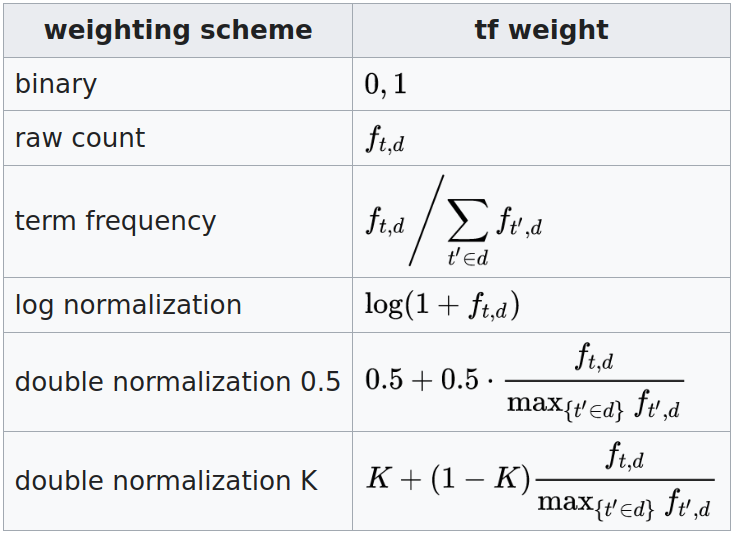
\includegraphics[width=13cm, angle=0]{Figures/VSM/variant-tf.png}}
	\end{center}
	\caption{Variant du TF \citep{sarch-engine-vsm}}
	\label{fig:variant-tf}
\end{figure}

\begin{figure}[htbp]
	\begin{center}
		\fbox{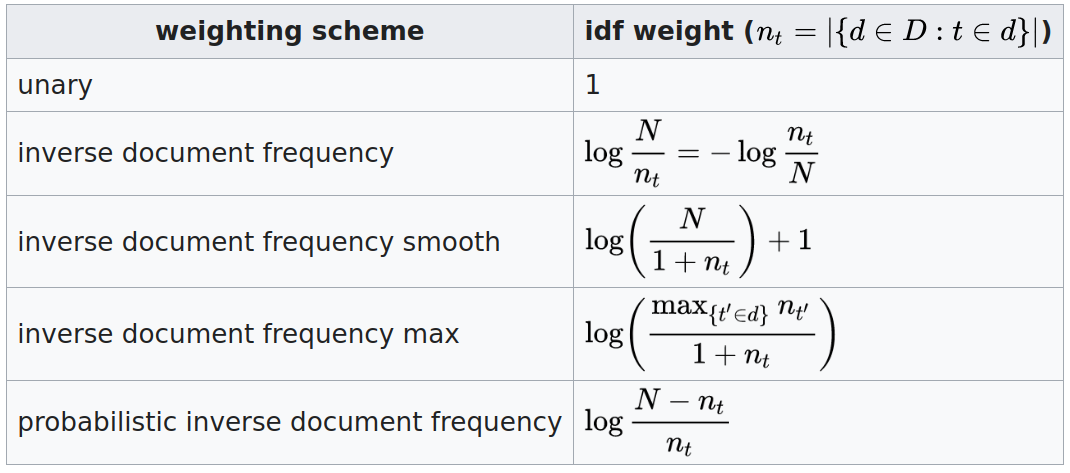
\includegraphics[width=15cm, angle=0]{Figures/VSM/variant-idf.png}}
	\end{center}
	\caption{Variant de l'IDF \citep{sarch-engine-vsm}}
	\label{fig:variant-idf}
\end{figure}

\begin{figure}[htbp]
	\begin{center}
		\fbox{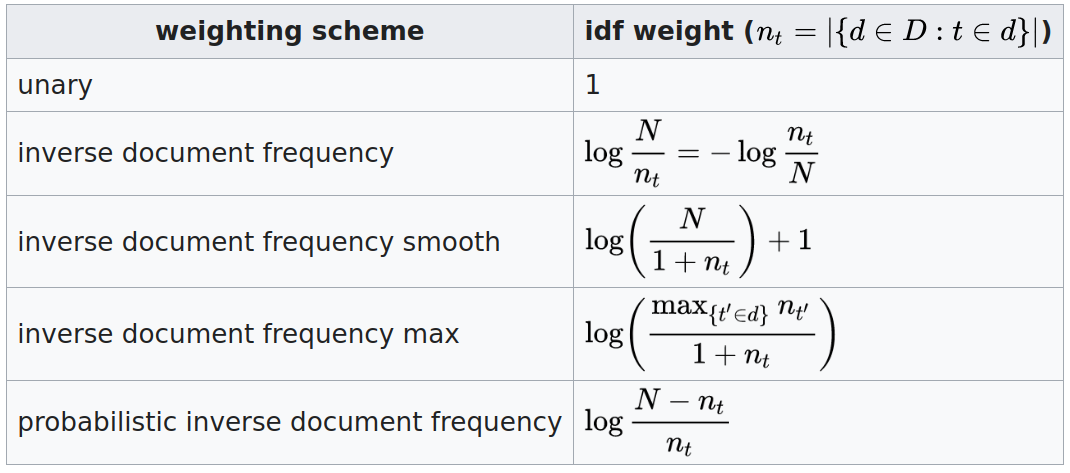
\includegraphics[width=15cm, angle=0]{Figures/VSM/variant-idf.png}}
	\end{center}
	\caption{Variant du TF-IDF \citep{sarch-engine-vsm}}
	\label{fig:variant-tf-idf}
\end{figure}

\section{Document inversé}
Le document inversé ou fichier inversé (Inverted index) permet de representer les documents ainsi que l'ensemble des termes dans la base de données, ainsi que ses poids calculés par ce méthode de pondération.

\section{Avantages}
Le modèle vectoriel a certains avantages: Facile a mettre en œuvre, possibilité d'avoir un appariement approximatif avec un degré de pertinence (L'utilisateur reçoit des documents qui pourrait lui intéressé), possibilité d'organiser les résultats suivant leur pertinence (L'utilisateur passe moins de temps a filtrer les résultats puisqu'ils sont déjà ordonné), ainsi ce modèle peut définir une limité pour la mesure de similarité et de n'afficher que les documents qui sont en dessus de cette limite pour éliminer les résultats le moins pertinent. Ce modèle est populaire, et plus utilisé par les moteurs de recherche actuel. \citep*{approche-semantique, modern-ir, soulier2014:def-evaluation-modele}

\section{Inconvénients}
Mais ce modèle a un inconvénients, qui est l’indépendance des termes d'indexation ce qui implique que la notion de sémantique du document est perdue. Mais ce problème a été solutionné par la mise place de regroupement des termes qui ont la même sens, on appelle N-grammes. Ou bien une autre approche est d'utiliser le modèle d’indexation sémantique latente (Latent Semantic Index).

\section{Conclusion}
Conclusion sur le VSM
\chapter{Réalisation}
\section{Approche utilisée}
\subsection{UML}
\lipsum[1-2]

\section{Technologies utilisé}
\subsection{Python}
\lipsum[1-2]

\subsection{MySQL}
\lipsum[1-2]

\section{Outils utilisée}
\lipsum[1-2]

\subsection{Visual Studio Code}
\lipsum[1-2]
\chapter{Conclusion}
\lipsum[15-20]

\renewcommand*{\mkbibnamefamily}[1]{\textsc{\textbf{#1}}}
\renewcommand*{\mkbibnameprefix}[1]{\textsc{\textbf{#1}}}

\begingroup
	\setlength\bibitemsep{5pt}
	\printbibliography[heading=bibintoc]
\endgroup

\end{document}